\documentclass[conference]{IEEEtran}
\IEEEoverridecommandlockouts

\usepackage{cite}
\usepackage{amsmath,amssymb,amsfonts}
\usepackage{booktabs}
\usepackage{graphicx}
\usepackage{textcomp}
\usepackage{xcolor}
\usepackage{hyperref}

\begin{document}

\title{SBi-FAGAT: Stance-Guided Bidirectional Frequency-Adaptive Graph Attention for Early Cascade Size and Polarization Prediction}

\author{
\IEEEauthorblockN{Vu Hieu Kien}
\IEEEauthorblockA{\textit{Faculty of Information Technology} \\
\textit{Thai Nguyen University of Information and Communication Technology (ICTU)}\\
Thai Nguyen, Vietnam}
\and
\IEEEauthorblockN{Vu Ngoc Anh Thuyen}
\IEEEauthorblockA{\textit{Faculty of Information Technology} \\
\textit{Thai Nguyen University of Information and Communication Technology (ICTU)}\\
Thai Nguyen, Vietnam}
}

\maketitle

\begin{abstract}
Predicting the eventual reach and community polarization of social media discussions from only the initial replies is challenging due to extreme early-stage sparsity, heterophilic conflict interactions, and asymmetric parent--child propagation dynamics. Existing rumor and cascade predictors predominantly rely on edge-sign-agnostic graph convolutions or post-hoc full-tree features that induce temporal leakage. Focusing specifically on \textbf{early cascade-level} (thread-level) stance dispersion and affective conflict rather than longitudinal user-network echo chambers, we present \textbf{SBi-FAGAT} (\emph{Stance-Guided Bidirectional Frequency-Adaptive Graph Attention Network}), a unified multi-task framework operating strictly on the source post and the earliest $K = 20$ chronological interactions. Our pipeline combines frozen \emph{Ancestor-Conditioned SpanPool} node embeddings and $10$-D causal structural-temporal descriptors with distilled 2D pairwise discourse attributes $e_{uv} = [s_{uv}, h_{uv}]^\top$ (ideological stance polarity separated from affective hostility) obtained from multilingual NLI stance verbalizers and class-weighted hostility teachers via reply-span-pooled cross-encoders. Inside the graph backbone, dual-channel Top-Down and Bottom-Up \texttt{StanceGuidedFAConv} layers pair signed frequency gates $\gamma_{uv} \in (-1, +1)$ with unsigned excitation gates, Dir-GNN bidirectional mixing, and root-aligned camp dipole readouts. Across inductive benchmarks on English PHEME and Vietnamese Reddit discussions, temporal holdout verification, leave-one-event-out evaluation, post-hoc text-free UPFD structural transfer, and observational edge-feature sensitivity analysis, SBi-FAGAT provides an interpretable, leakage-free framework verified against matched neural competitors, a non-learned Early-$K$ Persistence Baseline, RumourEval SDQC stance validation, and streamlined dual-annotator Vietnamese reliability audits.
\end{abstract}

\begin{IEEEkeywords}
Graph Neural Networks, Social Media Polarization, Information Cascades, Stance Detection, Early Prediction, Frequency-Adaptive Attention
\end{IEEEkeywords}

\section{Introduction}
Online information cascades frequently trigger rapid viral amplification alongside sharp ideological polarization. Forecasting both the ultimate cascade size $y_{\text{size}} = \ln(1 + N_{\text{total}})$ and future community polarization $y_{\text{polar}} \in [0, 1]$ before a thread matures enables proactive moderation and misinformation triage \cite{zubiaga2016analysing,li2017deepcas}. However, early prediction restricted strictly to the root post and the first $K=20$ interactions ($t \le t_K$) exposes three fundamental obstacles: (i) standard graph neural networks assume homophily (low-pass smoothing), erasing disagreement signals between conflicting commenters \cite{bo2021beyond,platonov2023critical}; (ii) unidirectional top-down convolutions ignore how reply subtrees synthesize conflict back toward the root \cite{bian2020rumor}; and (iii) unguarded feature engineering often leaks post-$t_K$ timestamps, tree depth statistics, or shared topic splits into early inputs.

To address these gaps within commodity 16~GB GPU and dual Tesla T4 budgets without sacrificing teacher coverage, we present a unified 2D architecture with the following contributions:
\begin{enumerate}
    \item \textbf{Leakage-Free Early Cascade Contract:} We formalize strict Parquet/PyG validation requiring UTC causality, fixed-horizon temporal normalization inside $t \le t_K$, forecasting eligibility ($N_{\text{reply}} \ge 25$), unified canonical topic splits (\texttt{topic\_splits.json}) shared across distillation, benchmark, and $K$-ablation subsets, and leave-one-out teacher edge isolation.
    \item \textbf{Ancestor-Conditioned SpanPool \& Reply-Span 2D Distillation:} Frozen bilingual social encoders (\texttt{uitnlp/visobert} \cite{nguyen2023visobert} for Vietnamese; \texttt{cardiffnlp/twitter-roberta-base} \cite{barbieri2020tweeteval} for English) extract contextual reply embeddings conditioned solely on causal ancestors (\texttt{[root, parent, reply]}). Pairwise $e_{uv} = [s_{uv}, h_{uv}]^\top$ teachers fuse a symmetric two-hypothesis \texttt{mDeBERTa-v3-xnli} stance verbalizer \cite{laurer2024less,he2023debertav3} with class-weighted hostility classifiers (\texttt{UIT-ViHSD} \cite{luu2021vihsd} / \texttt{TweetEval-Offensive} \cite{barbieri2020tweeteval}), distilling into a reply-span-pooled \texttt{DualHeadCrossEncoder}.
    \item \textbf{Dual-Channel Bidirectional SBi-FAGAT (\texttt{hidden\_dim=64}):} Two-stream node stems separate semantic embeddings from $10$-D causal topology descriptors, feeding Top-Down and Bottom-Up \texttt{StanceGuidedFAConv} stacks with explicit Dir-GNN cross-direction mixing \cite{rossi2023edge}, dual polarity/excitation message channels, and root-aligned BFS camp dipole readouts.
    \item \textbf{Multi-Faceted Scientific Verification:} Beyond fixed-hyperparameter comparison against seven matched neural baselines (\texttt{hidden\_dim=64}, symmetric uncertainty prediction, and shared causal Persistence-Residual anchoring for stance-aware architectures) plus a matched \texttt{BiEdgeGATv2} ablation comparator, we evaluate non-learned Early-$K$ Persistence, Sarle's Bimodality Coefficient \cite{pfister2013good}, signed assortativity, Vietnamese temporal holdout (\texttt{edge\_source="teacher"}), post-hoc text-free UPFD \cite{dou2021upfd} structural transfer via \texttt{LatentConflictMLP}, RumourEval SDQC and Vietnamese dual-annotator pair/thread reliability audits, and observational edge-feature sensitivity analysis.
\end{enumerate}

\section{Related Work}
\subsection{Graph Neural Networks for Cascades and Heterophily}
Conventional GCN \cite{kipf2017semisupervised} and dynamic GATv2 \cite{brody2022how} aggregate neighborhood features via strictly positive weights, acting as low-pass filters that degrade when adjacent nodes hold opposing viewpoints \cite{platonov2023critical}. Bi-GCN \cite{bian2020rumor} introduced bidirectional top-down and bottom-up propagation with root enhancement for rumor detection, Dir-GNN \cite{rossi2023edge} demonstrated that decoupling directed message directions improves learning on heterophilic graphs, and FAGCN \cite{bo2021beyond} and Signed GCN \cite{derr2018signed} introduced negative edge weights to separate low- and high-frequency components. SBi-FAGAT unifies directional tree asymmetry with explicitly NLP-guided continuous 2D edge vectors $e_{uv}$, symmetric activations, and root-aligned dipole pooling.

\subsection{NLP Stance Detection and Controversy Quantification}
Discourse stance benchmarks such as PHEME \cite{zubiaga2016analysing,kochkina2018pheme} and RumourEval-2019 \cite{gorrell2019semeval} classify replies relative to claims. Multilingual NLI transfer \cite{laurer2024less}, social hate/offensive detection \cite{barbieri2020tweeteval,luu2021vihsd}, and DeBERTaV3 \cite{he2023debertav3} / ViSoBERT \cite{nguyen2023visobert} backbones provide domain-adapted discourse representations. Because random-walk controversy metrics such as RWC \cite{garimella2016quantifying,garimella2018quantifying} degenerate on sparse shallow trees ($|\mathcal{V}_K| \le 21$), we quantify polarization via continuous root-aligned future stance dispersion verified against Sarle's Bimodality Coefficient \cite{pfister2013good} and signed assortativity.

\section{Methodology}
\subsection{Problem Formulation and Zero-Leakage Protocol}
Given a propagation tree observed up to the earliest $K=20$ chronological replies $\mathcal{G}_K = (\mathcal{V}_K, \mathcal{E}_K^{\text{TD}}, \mathcal{E}_K^{\text{BU}})$, each node $v \in \mathcal{V}_K$ carries a $770$-D feature vector $x_v = [\mathbf{e}_v^{\text{Span}} \Vert t_{\text{norm}}(v) \Vert d_{\text{norm}}(v)]$ paired with a $10$-D causal structural vector $s_v \in [0, 1]^{10}$ and an $8$-D cascade summary vector $c_{\mathcal{G}}$ (all computed strictly from $t \le t_K$). Post-observation replies ($t > t_K$, count $n \ge 2$) define targets:
\begin{equation}
y_{\text{size}} = \ln(1 + N_{\text{total}}), \quad
y_{\text{polar}} = \operatorname{clip}\!\left(\lambda_p \min\!\left(1, \sqrt{\min(1, s_{\tilde{s}, \text{ddof}=1}^2)}\right) + (1-\lambda_p)\min\!\left(1, 2\sqrt{\frac{n}{n-1} m_+ m_-}\right), 0, 1\right),
\end{equation}
where $\lambda_p = 0.5$, $\tilde{s}_v \in [-1, 1]$ denotes root-aligned future stances over $t > t_K$ (\texttt{future\_only}), $m_+ = \frac{1}{n}\sum_v \max(\tilde{s}_v, 0)$ and $m_- = \frac{1}{n}\sum_v \max(-\tilde{s}_v, 0)$ are continuous camp intensities whose finite-sample covariance bias is removed prior to square-root linear amplitude scaling and $[0, 1]$ clipping by $\frac{n}{n-1}$ (preventing quadratic collapse on empirical cascades), and PHEME cascades additionally supervise $y_{\text{rumor}}$. Forecasting splits require $N_{\text{reply}} \ge 25$ (with optional $K=10, N_{\text{reply}} \ge 15$ evaluation on sparser PHEME events) so non-trivial future evolution exists. Topic splits partition Train/Val/Test (70\%/15\%/15\%) canonically across news events (PHEME) or via a \emph{Heuristic Temporal-Keyword / 30-day TF-IDF ($\cos \ge 0.30$) Grouped Inductive Split} (Vietnamese Reddit, alongside chronological temporal holdout with \texttt{edge\_source="teacher"}), persisting \texttt{topic\_splits.json} so distillation, evaluation, and fixed-horizon $K \in \{10, 20, 30, 50\}$ sensitivity runs never re-split Train topics into Test.

\subsection{Offline Ancestor-Conditioned SpanPool and 2D Distillation}
To decouple transformer memory from multi-seed GNN sweeps, node embeddings and edge scores are precomputed offline in mixed precision (\texttt{FP16}). For node embeddings $\mathbf{e}_v^{\text{Span}} \in \mathbb{R}^{768}$, frozen encoders (\texttt{uitnlp/visobert} for VI, \texttt{cardiffnlp/twitter-roberta-base} for EN) process causal context sequences \texttt{[CLS] root [SEP] parent [SEP] reply [SEP]} (with 60/40 head--tail root truncation) and mean-pool exclusively over reply tokens, disambiguating short replies without accessing future nodes.

For 2D edge attributes $e_{uv} = [s_{uv}, h_{uv}]^\top \in [-1, 1] \times [0, 1]$:
\begin{itemize}
    \item \textbf{Symmetric NLI Stance Teacher ($s_{uv}$):} Within a 384-token budget preserving the full reply span, \texttt{mDeBERTa-v3-base-xnli} evaluates two symmetric hypotheses (support vs.\ opposition) over parent--reply pairs, attributing double contradictions $\min(c_{\text{sup}}, c_{\text{opp}})$ to neutral on the 3-class stance simplex so $s_{uv} = P(\text{support}) - P(\text{oppose})$.
    \item \textbf{Class-Weighted Hostility Teacher ($h_{uv}$):} Inverse-frequency square-root class weighting fine-tunes \texttt{uitnlp/visobert} on \texttt{UIT-ViHSD} \cite{luu2021vihsd} (VI), paired with \texttt{twitter-roberta-base-offensive} \cite{barbieri2020tweeteval} (EN).
    \item \textbf{Reply-Span-Pooled Student (\texttt{DualHeadCrossEncoder}):} Trained strictly on $\mathcal{T}_{\text{train}}$ with a 5-block relational interaction vector $[h_{\text{CLS}} \Vert h_{\text{ctx}} \Vert h_{\text{reply}} \Vert h_{\text{ctx}} \odot h_{\text{reply}} \Vert |h_{\text{ctx}} - h_{\text{reply}}|]$ for stance and reply-span pooling for $h_{uv}$ (attenuating parent profanity bleed into clean replies), temperature-scaled KL ($T=2.0$) + $0.5\,\text{SmoothL1}$ + \texttt{BCEWithLogitsLoss}, deep \texttt{(root, reply)} pairs, differential AdamW learning rates, and LOO \texttt{edge\_source="teacher"} isolation.
\end{itemize}

\subsection{Dual-Channel Bidirectional SBi-FAGAT Architecture}
A shared \texttt{TwoStreamNodeStem} projects semantic and $10$-D causal structural inputs into $h^{(0)} \in \mathbb{R}^{64}$ (masking topology columns in both \texttt{struct\_x} and \texttt{cascade\_stats} for \texttt{TextMLP}). Each \texttt{StanceGuidedFAConv} layer normalizes linear node projections $z^{\text{norm}} = \operatorname{LN}(W h^{(l-1)})$ and evaluates scaled node--edge gates (with node-attention Xavier gain $0.2$ and initial cosine weight $\omega^{(0)} = 0.10$):
\begin{equation}
\gamma_{uv} = \tanh\!\left(\frac{\mathbf{a}_{\text{node}}^\top [z_u^{\text{norm}} \Vert z_v^{\text{norm}}]}{\sqrt{2d}} + \omega \cos(z_u^{\text{norm}}, z_v^{\text{norm}}) + \mathbf{a}_{\text{edge}}^\top e_{uv} + \delta_{\gamma}(e_{uv})\right),
\end{equation}
alongside an unsigned excitation gate $\alpha_{uv}^{\text{exc}} = \sigma(0.8|s_{uv}| + 0.8 h_{uv} + \delta_{\alpha}(e_{uv}))$. Messages split evenly into signed polarity ($\gamma_{uv} z_u[:d/2]$) and unsigned excitation ($\alpha_{uv}^{\text{exc}} z_u[d/2:]$) channels under symmetric degree normalization $c_{uv} = \sqrt{(d_{\text{out}}(u)+1)(d_{\text{in}}(v)+1)}$, updated with initial residual anchoring ($0.5 h^{(l-1)} + \epsilon h^{(0)} + m_v + W_{\text{root}} h_r^{(0)}$) and odd-symmetric stabilization $r + 0.2\tanh(r)$. After each layer, Dir-GNN cross-mixing ($\eta_l^{(0)} = 0.10$) \cite{rossi2023edge} couples TD and BU states ($\tilde{h}^{\delta} = h^{\delta} + \tanh(\eta_l) W_{\text{mix}}^{\delta} h^{\bar{\delta}}$). Finally, base pooling $z_{\text{base}} = [z_{\text{root}} \Vert z_{\text{att}}]$ is modulated by a residual CleanRes Camp Dipole bottleneck $\operatorname{dipole\_proj}: \mathbb{R}^{3d+6} \to \mathbb{R}^{\max(16, d/2)} \to \mathbb{R}^{2d}$ scaled by $\tanh(\beta_{\text{dip}})$ ($\beta_{\text{dip}}^{(0)} = 0.25$) over node dispersion $z_{\text{disp}}$, BFS root-aligned camp dipoles up to $64$ hops (detached parent ramp $\operatorname{clip}(u_{\text{ori}}/0.1, -1, 1)$, continuous ReLU camp weights $w_\pm = \operatorname{ReLU}(\pm\hat{\gamma}_{uv})$, masked camp centroids $\mu_\pm = \mathbb{I}[\sum w_\pm > 10^{-6}]\frac{\sum w_\pm h_v}{\max(\sum w_\pm, 10^{-6})}$, dual-camp indicator $b = 2\,\mathbb{I}[\text{both\_camps}]\sqrt{\operatorname{clip}(f_+ f_-, 0, 0.25) + 10^{-8}}$, yielding zeroed single-camp vectors $z_{\text{dipole}}^{\text{polar}} = b\sqrt{(\mu_+ - \mu_-)^2 \mathbb{I}[\text{both\_camps}] + 10^{-8}}$ and $z_{\text{dipole}}^{\text{signed}} = (\mu_+ - \mu_-)\mathbb{I}[\text{both\_camps}]$), and 6 scalar gate moments before $\operatorname{LN}(z_{\text{base}} + \tanh(\beta_{\text{dip}})\,\operatorname{dipole\_proj}(\cdot))$. Inside \texttt{MultiTaskHead}, \texttt{polar\_head} reads strictly from $2d$-D \texttt{graph\_emb} across all compared architectures, decoupling polarization inference from $8$-D \texttt{cascade\_stats}; for all stance-aware models consuming explicit edge stances (\texttt{TemporalStanceMLP}, non-latent \texttt{EdgeGATv2}, \texttt{BiEdgeGATv2}, and non-ablated \texttt{SBiFAGAT}), logits add a learnable causal Persistence-Residual anchor $z_{\text{polar}} = \tanh(w_p)\bigl(\operatorname{logit}(\operatorname{clip}(y_{\text{polar}}(\mathcal{G}_K), 0.02, 0.98)) - \bar{\ell}_{\text{train}}\bigr) + \Delta z_{\text{polar}}$.

\subsection{Multi-Task Optimization}
To prevent sigmoid tail gradient starvation on $y_{\text{polar}}$, we replace raw sigmoid Huber loss with zero-minimum KL-calibrated binary cross-entropy over logits $z_{\text{polar}}$ combined with Smooth-L1 regression ($\beta=0.05$):
\begin{equation}
\mathcal{L}_{\text{polar}} = \bigl(\operatorname{BCEWithLogits}(z_{\text{polar}}, y_{\text{polar}}) - H(y_{\text{polar}})\bigr)_+ + \operatorname{SmoothL1}(\sigma(z_{\text{polar}}), y_{\text{polar}}),
\end{equation}
jointly with Huber loss on $y_{\text{size}}$ and masked dampened class-weighted Cross-Entropy on $y_{\text{rumor}}$. Training applies strictly train-only 2:1 constant-mean baseline-normalized loss scaling ($s_{\text{size}}, s_{\text{polar}}$) and calibrated output bias initialization ($p \in [10^{-3}, 0.99]$), symmetric uncertainty prediction across all 8 architectures when enabled, paired per-seed DataLoader shuffle ordering, linear warmup followed by \texttt{ReduceLROnPlateau}, Exponential Moving Average (EMA) validation selection, Early Stopping on validation task loss, validation-only comparator model selection (\texttt{val\_summary\_stats}), and $R^2_{\text{polar}}$ reporting across five deterministic seeds ($[42, 100, 2024, 777, 999]$).

\section{Experimental Setup}
All experiments evaluate 8 architectures fairly at fixed shared hyperparameters (\texttt{hidden\_dim=64}, matching $128$-D regression heads) alongside the non-learned Early-$K$ Persistence Baseline across 5 deterministic seeds, reporting paired $t$-tests, sample/topic-cluster paired bootstrap $p$-values (and exact sign-flip permutation tests for $F < 6$ LOO folds), and Holm--Bonferroni adjusted direction-aware significance against the strongest learned comparator. \IfFileExists{tables_dataset_eda.tex}{Table~\ref{tab:dataset_eda}}{\IfFileExists{tables_dataset_eda_pheme.tex}{Table~\ref{tab:dataset_eda_pheme}\IfFileExists{tables_dataset_eda_vn.tex}{ and Table~\ref{tab:dataset_eda_vn}}{}}{\IfFileExists{tables_dataset_eda_vn.tex}{Table~\ref{tab:dataset_eda_vn}}{Table~\ref{tab:dataset_eda}}}} reports dataset splits and Early-$K$ Persistence statistics generated directly from validated Parquet tables.

\IfFileExists{tables_dataset_eda.tex}{
  \begin{table*}[t]
\centering
\caption{Exploratory dataset statistics ($K=20$, $N_{\text{reply}} \ge 25$ forecasting filter) and Early-$K$ Persistence Baseline on Test splits.}
\label{tab:dataset_eda}
\resizebox{\textwidth}{!}{
\begin{tabular}{lcccccccc}
\toprule
Dataset & Raw & Forecast ($\ge 25$) & Topics & Train/Val/Test & Med (Mean) Replies & Med Span (h) & Persist RMSE$\downarrow$ & Persist $r$$\uparrow$ \\
\midrule
pheme & 6,425 & 874 & 6 & 570/228/76 & 11.0 (14.8) & 2.53 & 0.0161 & 0.2954 \\
vn & 1,500 & 1,500 & 1,496 & 1050/225/225 & 44.0 (57.5) & 95.22 & 0.0788 & 0.0217 \\
\bottomrule
\end{tabular}
}
\end{table*}

}{
  \IfFileExists{tables_dataset_eda_pheme.tex}{
    \begin{table*}[t]
\centering
\caption{Exploratory dataset statistics ($K=20$, $N_{\text{reply}} \ge 25$ forecasting filter) and Early-$K$ Persistence Baseline on Test splits.}
\label{tab:dataset_eda_pheme}
\resizebox{\textwidth}{!}{
\begin{tabular}{lcccccccc}
\toprule
Dataset & Raw & Forecast ($\ge 25$) & Topics & Train/Val/Test & Med (Mean) Replies & Med Span (h) & Persist RMSE$\downarrow$ & Persist $r$$\uparrow$ \\
\midrule
pheme & 6,425 & 874 & 6 & 570/228/76 & 11.0 (14.8) & 2.53 & 0.0161 & 0.2954 \\
\bottomrule
\end{tabular}
}
\end{table*}

  }{}
  \IfFileExists{tables_dataset_eda_vn.tex}{
    \begin{table*}[t]
\centering
\caption{Exploratory dataset statistics ($K=20$, $N_{\text{reply}} \ge 25$ forecasting filter) and Early-$K$ Persistence Baseline on Test splits.}
\label{tab:dataset_eda_vn}
\resizebox{\textwidth}{!}{
\begin{tabular}{lcccccccc}
\toprule
Dataset & Raw & Forecast ($\ge 25$) & Topics & Train/Val/Test & Med (Mean) Replies & Med Span (h) & Persist RMSE$\downarrow$ & Persist $r$$\uparrow$ \\
\midrule
vn & 1,500 & 1,500 & 1,496 & 1050/225/225 & 44.0 (57.5) & 95.22 & 0.0231 & 0.0745 \\
\bottomrule
\end{tabular}
}
\end{table*}

  }{
    \IfFileExists{tables_dataset_eda_pheme.tex}{}{
      \begin{table}[t]
      \centering
      \caption{Dataset EDA and Early-$K$ Persistence Baseline (pending \texttt{scripts/export\_dataset\_stats.py} execution on processed datasets).}
      \label{tab:dataset_eda}
      \begin{tabular}{lc}
      \toprule
      Artifact & Status \\
      \midrule
      \texttt{tables\_dataset\_eda.tex} & Pending corpus execution \\
      \bottomrule
      \end{tabular}
      \end{table}
    }
  }
}

\section{Results and Ablation Studies}
This manuscript template strictly forbids pre-filled or synthetic metric numbers; all empirical values below are read directly from validated pipeline outputs. On the 225-cascade Vietnamese Reddit Test split ($1,500$ eligible cascades / $1,496$ heuristic topics; \texttt{future\_only} linear-amplitude target, $K=20, N_{\text{reply}} \ge 25$), the non-learned Early-$K$ Persistence Baseline yields RMSE $= 0.0788$, $R^2_{\text{polar}} = -3.1986$, Pearson $r = 0.0217$, and Spearman $\rho = 0.0363$, confirming that early-window variance alone poorly predicts post-$K$ polarization dynamics. In the 5-seed v3 canonical VN benchmark (Table~\ref{tab:main_vn}), ReZero zero-initialized Persistence-Residual anchoring eliminates negative-$R^2$ collapse across stance-aware architectures: SBi-FAGAT achieves the lowest polarization RMSE ($0.0370 \pm 0.0003$) and highest $R^2_{\text{polar}}$ ($0.0742 \pm 0.0157$, $r = 0.2899 \pm 0.0278$, $\rho = 0.2272 \pm 0.0176$), closely trailed by \texttt{TextMLP} ($0.0370 \pm 0.0004$, $R^2_{\text{polar}} = 0.0741 \pm 0.0181$, $r = 0.2989 \pm 0.0110$), \texttt{EdgeGATv2} ($R^2_{\text{polar}} = 0.0689 \pm 0.0206$), and validation-selected comparator \texttt{TemporalStanceMLP} ($R^2_{\text{polar}} = 0.0608 \pm 0.0239$; Holm--Bonferroni adjusted $p_{\text{adj}} \ge 0.574$, showing statistically comparable headline accuracy on $K=20$ VN alongside \texttt{StandardGCN} at lowest size MSLE $0.1542 \pm 0.0048$). Under chronological VN temporal holdout (\texttt{split\_mode="temporal"}, \texttt{edge\_source="teacher"}, $225$ Test cascades; Table~\ref{tab:temporal_vn}), Early-$K$ Persistence degrades to $R^2_{\text{polar}} = -5.4386$ (RMSE $= 0.0874$, $r = 0.1778$, $\rho = 0.1741$), whereas all learned architectures generalize with strictly positive $R^2_{\text{polar}} \in [0.0481, 0.0815]$: \texttt{SBiFAGAT} attains the strongest rank correlation ($\rho = 0.3058 \pm 0.0187$, RMSE $= 0.0334 \pm 0.0009$, $r = 0.3338 \pm 0.0319$), validation-selected \texttt{TemporalStanceMLP} reaches $R^2_{\text{polar}} = 0.0815 \pm 0.0198$ ($r = 0.3377 \pm 0.0112$, RMSE $= 0.0330 \pm 0.0004$; Holm--Bonferroni $p_{\text{adj}} = 1.00$), and \texttt{FAGCN} leads size prediction (MSLE $= 0.1881 \pm 0.0129$, $R^2_{\text{size}} = 0.2586 \pm 0.0509$). In the refreshed 5-seed v3 ReZero VN component ablation (Table~\ref{tab:ablation_vn}), \texttt{SBiFAGAT (Full)} achieves MSLE $= 0.1580 \pm 0.0070$, $R^2_{\text{size}} = 0.2925 \pm 0.0315$, RMSE $= 0.0369 \pm 0.0003$, $R^2_{\text{polar}} = 0.0777 \pm 0.0141$, $r = 0.2939 \pm 0.0223$, and $\rho = 0.2335 \pm 0.0180$, remaining statistically comparable to matched \texttt{BiEdgeGATv2 (Matched)} ($R^2_{\text{polar}} = 0.0789 \pm 0.0172$, Holm--Bonferroni $p_{\text{adj}} = 1.00$); ablating Camp Dipole \& Moments ($R^2_{\text{polar}} = 0.0503 \pm 0.0208$) or the signed Conflict Gate ($0.0527 \pm 0.0258$) causes the largest drops in polarization explained variance, while removing 8-D Burst Stats cuts $R^2_{\text{size}}$ from $0.2925$ to $0.2215 \pm 0.0429$. On the fixed-future common subset ($N_{\text{reply}} \ge 55$, future window $k > 50$; Fig.~\ref{fig:k_curve_vn}), \texttt{SBiFAGAT} size MSLE tightens monotonically from $0.1443$ ($K=10$) to $0.1370$ ($K=20$), $0.1352$ ($K=30$), and $0.1053$ ($K=50$, $R^2_{\text{size}} = 0.2882$), with polarization correlation rising from $r = 0.2523$ ($\rho = 0.1813$) at $K=10$ to $r = 0.2921$ ($\rho = 0.2346$) at $K=20$ and $r = 0.2882$ ($\rho = 0.2362$) at $K=50$. In observational VN Test sensitivity analysis (Table~\ref{tab:mechanisms_vn}), early hostility correlates modestly with cascade size ($\rho = 0.2128, r = 0.2044$) and early stance spread with future polarization ($r = 0.1593$), while neutralizing all early opposition shifts predicted polarization by $\Delta \hat{y}_{\text{polar}} = -0.0035$ overall ($-0.0037$ on Q75+ cascades). Locally profiled VN CPU inference requires $1.1721$\,ms/cascade across $137,086$ parameters ($0.03$\,MB peak allocated RAM), complementing Table~\ref{tab:efficiency}. Optional Track 2 PHEME Tier 2A ($K=10, N_{\text{reply}} \ge 15$) multi-seed re-execution requires re-extracting \texttt{pheme/nlp\_features.pt} with \texttt{min\_total\_replies=15} because the existing archive was extracted at \texttt{min\_total\_replies\_extracted=25} (legacy Cohort B); accordingly, existing \texttt{tables\_*\_pheme.tex} reflect legacy Cohort B, UPFD tables report post-hoc text-free structural transfer, and blind VN Gate 1 audit sheets ($20$ pilot / $120$ pairs / $30$ trees) are exported and sealed pending manual annotation.

\IfFileExists{tables_main_pheme.tex}{
  \begin{table*}[t]
\centering
\caption{Early Cascade Size, Polarization, and Rumor Prediction at $K=20$ (INDUCTIVE, Mean $\pm$ Std). Stars indicate significance vs. EdgeGATv2 ($^{*}p<0.05$, $^{**}p<0.01$).}
\label{tab:main_pheme}
\resizebox{\textwidth}{!}{
\begin{tabular}{lcccccccc}
\toprule
Model & MSLE $\downarrow$ & MAE $\downarrow$ & $R^2_{\text{size}}$ $\uparrow$ & RMSE $\downarrow$ & Pearson $r$ $\uparrow$ & Spearman $\rho$ $\uparrow$ & Macro-F1 $\uparrow$ & Acc $\uparrow$ \\
\midrule
Early-K Persistence & 0.1186 $\pm$ 0.0000 & 0.2968 $\pm$ 0.0000 & -0.2136 $\pm$ 0.0000 & 0.0161 $\pm$ 0.0000 & 0.2954 $\pm$ 0.0000 & \textbf{0.4241 $\pm$ 0.0000} & -- & -- \\
TextMLP & 0.1075 $\pm$ 0.0190 & 0.2747 $\pm$ 0.0298 & -0.1008 $\pm$ 0.1943 & 0.0127 $\pm$ 0.0002 & 0.2156 $\pm$ 0.0479 & 0.1857 $\pm$ 0.0720 & 0.2750 $\pm$ 0.0565 & 0.4895 $\pm$ 0.0686 \\
TemporalStanceMLP & 0.0967 $\pm$ 0.0046 & 0.2505 $\pm$ 0.0103 & 0.0097 $\pm$ 0.0472 & 0.0126 $\pm$ 0.0002 & 0.1867 $\pm$ 0.0416 & 0.1625 $\pm$ 0.0267 & 0.3156 $\pm$ 0.0746 & \textbf{0.5763 $\pm$ 0.1004} \\
StandardGCN & \textbf{0.0928 $\pm$ 0.0065} & 0.2455 $\pm$ 0.0180 & \textbf{0.0498 $\pm$ 0.0664} & 0.0129 $\pm$ 0.0002 & 0.1690 $\pm$ 0.0455 & 0.1118 $\pm$ 0.0439 & 0.3010 $\pm$ 0.0698 & 0.5526 $\pm$ 0.0335 \\
StandardGATv2 & 0.1042 $\pm$ 0.0057 & 0.2636 $\pm$ 0.0187 & -0.0665 $\pm$ 0.0588 & 0.0129 $\pm$ 0.0003 & 0.2117 $\pm$ 0.0509 & 0.1635 $\pm$ 0.0408 & 0.3212 $\pm$ 0.0580 & 0.5763 $\pm$ 0.0845 \\
EdgeGATv2 & 0.0942 $\pm$ 0.0060 & \textbf{0.2436 $\pm$ 0.0193} & 0.0353 $\pm$ 0.0610 & 0.0127 $\pm$ 0.0003 & 0.2170 $\pm$ 0.0628 & 0.1960 $\pm$ 0.0708 & 0.3103 $\pm$ 0.0620 & 0.5553 $\pm$ 0.0606 \\
FAGCN & 0.1116 $\pm$ 0.0228 & 0.2798 $\pm$ 0.0388 & -0.1424 $\pm$ 0.2338 & 0.0126 $\pm$ 0.0002 & 0.2295 $\pm$ 0.0691 & 0.1746 $\pm$ 0.0856 & 0.3327 $\pm$ 0.0297 & 0.5553 $\pm$ 0.0487 \\
BiGCN & 0.1145 $\pm$ 0.0206 & 0.2766 $\pm$ 0.0321 & -0.1716 $\pm$ 0.2109 & 0.0128 $\pm$ 0.0003 & 0.2228 $\pm$ 0.0358 & 0.1849 $\pm$ 0.0522 & \textbf{0.3411 $\pm$ 0.0806} & 0.5553 $\pm$ 0.0995 \\
SBiFAGAT & 0.1062 $\pm$ 0.0090 & 0.2652 $\pm$ 0.0120 & -0.0867 $\pm$ 0.0923 & \textbf{0.0124 $\pm$ 0.0002}$^{*}$ & \textbf{0.3001 $\pm$ 0.0542} & 0.2186 $\pm$ 0.0504 & 0.3062 $\pm$ 0.0493 & 0.5605 $\pm$ 0.0748 \\
\midrule
$p$-value (SBiFAGAT vs. EdgeGATv2) & 5.45e-02 & 1.09e-01 & 5.45e-02 & 9.26e-02 & 1.32e-01 & 6.61e-01 & 9.38e-01 & 9.28e-01 \\
Bootstrap $p$ (SBiFAGAT vs. EdgeGATv2) & 7.64e-02 & 2.16e-02 & 7.76e-02 & 3.20e-03 & 4.72e-02 & 5.55e-01 & 7.75e-01 & 8.56e-01 \\
Holm-Bonferroni $p$ (SBiFAGAT vs. EdgeGATv2) & 4.36e-01 & 5.55e-01 & 4.36e-01 & 5.55e-01 & 5.55e-01 & 1.00e+00 & 1.00e+00 & 1.00e+00 \\
Holm-Bonf Bootstrap $p$ (SBiFAGAT vs. EdgeGATv2) & 3.82e-01 & 1.51e-01 & 3.82e-01 & 2.56e-02 & 2.83e-01 & 1.00e+00 & 1.00e+00 & 1.00e+00 \\
\bottomrule
\end{tabular}
}
\end{table*}

}{
  \begin{table}[t]
  \centering
  \caption{PHEME 5-Seed Inductive Benchmark Comparison (pending GPU run of \texttt{scripts/run\_experiments.py}).}
  \label{tab:main_pheme}
  \begin{tabular}{lc}
  \toprule
  Artifact & Status \\
  \midrule
  \texttt{tables\_main\_pheme.tex} & Pending 5-seed execution \\
  \bottomrule
  \end{tabular}
  \end{table}
}

\IfFileExists{tables_loo_pheme.tex}{
  \begin{table*}[t]
\centering
\caption{Early Cascade Size, Polarization, and Rumor Prediction at $K=20$ (LOO, Mean $\pm$ Std). Stars indicate significance vs. TemporalStanceMLP ($^{*}p<0.05$, $^{**}p<0.01$).}
\label{tab:loo_pheme}
\resizebox{\textwidth}{!}{
\begin{tabular}{lcccccccc}
\toprule
Model & MSLE $\downarrow$ & MAE $\downarrow$ & $R^2_{\text{size}}$ $\uparrow$ & RMSE $\downarrow$ & Pearson $r$ $\uparrow$ & Spearman $\rho$ $\uparrow$ & Macro-F1 $\uparrow$ & Acc $\uparrow$ \\
\midrule
Early-K Persistence & 0.1803 $\pm$ 0.0551 & 0.3356 $\pm$ 0.0381 & -0.4895 $\pm$ 0.9933 & 0.0165 $\pm$ 0.0045 & \textbf{0.2572 $\pm$ 0.1111} & \textbf{0.3851 $\pm$ 0.1219} & -- & -- \\
TextMLP & 0.1756 $\pm$ 0.0875 & 0.3064 $\pm$ 0.0609 & -0.2485 $\pm$ 0.4359 & 0.0127 $\pm$ 0.0026 & 0.1720 $\pm$ 0.0823 & 0.1380 $\pm$ 0.1155 & 0.2836 $\pm$ 0.0468 & 0.6298 $\pm$ 0.1678 \\
TemporalStanceMLP & 0.1661 $\pm$ 0.0817 & \textbf{0.2949 $\pm$ 0.0594} & -0.1661 $\pm$ 0.3575 & 0.0127 $\pm$ 0.0027 & 0.1808 $\pm$ 0.0523 & 0.1212 $\pm$ 0.0964 & 0.2831 $\pm$ 0.0645 & 0.6171 $\pm$ 0.1695 \\
StandardGCN & 0.1804 $\pm$ 0.0809 & 0.3140 $\pm$ 0.0508 & -0.3057 $\pm$ 0.4190 & 0.0128 $\pm$ 0.0027 & 0.1509 $\pm$ 0.0235 & 0.1202 $\pm$ 0.0942 & 0.2675 $\pm$ 0.0544 & 0.6076 $\pm$ 0.1637 \\
StandardGATv2 & 0.1704 $\pm$ 0.0872 & 0.2990 $\pm$ 0.0620 & -0.1809 $\pm$ 0.3275 & 0.0127 $\pm$ 0.0027 & 0.1822 $\pm$ 0.0349 & 0.1321 $\pm$ 0.1129 & 0.2760 $\pm$ 0.0489 & 0.6192 $\pm$ 0.1641 \\
EdgeGATv2 & 0.1769 $\pm$ 0.0877 & 0.3069 $\pm$ 0.0614 & -0.2230 $\pm$ 0.2921 & \textbf{0.0126 $\pm$ 0.0026} & 0.1562 $\pm$ 0.1169 & 0.1281 $\pm$ 0.1472 & 0.2983 $\pm$ 0.0590 & 0.6219 $\pm$ 0.1480 \\
FAGCN & 0.1676 $\pm$ 0.0811 & 0.2997 $\pm$ 0.0632 & -0.1795 $\pm$ 0.3520 & 0.0128 $\pm$ 0.0026 & 0.1480 $\pm$ 0.1069 & 0.1241 $\pm$ 0.1463 & 0.2846 $\pm$ 0.0620 & 0.6201 $\pm$ 0.1595 \\
BiGCN & 0.1747 $\pm$ 0.0795 & 0.3084 $\pm$ 0.0493 & -0.2678 $\pm$ 0.4689 & 0.0128 $\pm$ 0.0026 & 0.1805 $\pm$ 0.0312 & 0.1206 $\pm$ 0.1021 & \textbf{0.2991 $\pm$ 0.0394} & \textbf{0.6452 $\pm$ 0.1437} \\
SBiFAGAT & \textbf{0.1651 $\pm$ 0.0787} & 0.2959 $\pm$ 0.0582 & \textbf{-0.1578 $\pm$ 0.3365} & 0.0128 $\pm$ 0.0025 & 0.1960 $\pm$ 0.0687 & 0.1519 $\pm$ 0.0672 & 0.2912 $\pm$ 0.0698 & 0.6306 $\pm$ 0.1392 \\
\midrule
$p$-value (SBiFAGAT vs. TemporalStanceMLP) & 8.05e-01 & 6.33e-01 & 6.68e-01 & 6.11e-01 & 6.21e-01 & 1.75e-01 & 8.15e-01 & 6.71e-01 \\
Exact Perm. $p$ (SBiFAGAT vs. TemporalStanceMLP) & 8.12e-01 & 6.88e-01 & 6.88e-01 & 1.00e+00 & 6.88e-01 & 1.88e-01 & 8.12e-01 & 6.88e-01 \\
Holm-Bonferroni $p$ (SBiFAGAT vs. TemporalStanceMLP) & 1.00e+00 & 1.00e+00 & 1.00e+00 & 1.00e+00 & 1.00e+00 & 1.00e+00 & 1.00e+00 & 1.00e+00 \\
Holm-Bonf Exact Perm. $p$ (SBiFAGAT vs. TemporalStanceMLP) & 1.00e+00 & 1.00e+00 & 1.00e+00 & 1.00e+00 & 1.00e+00 & 1.00e+00 & 1.00e+00 & 1.00e+00 \\
\bottomrule
\end{tabular}
}
\end{table*}

}{}

\IfFileExists{tables_main_vn.tex}{
  \begin{table*}[t]
\centering
\caption{Early Cascade Size, Polarization, and Rumor Prediction at $K=20$ (INDUCTIVE, Mean $\pm$ Std). Stars indicate significance vs. TemporalStanceMLP ($^{*}p<0.05$, $^{**}p<0.01$).}
\label{tab:main_vn}
\resizebox{\textwidth}{!}{
\begin{tabular}{lcccccc}
\toprule
Model & MSLE $\downarrow$ & MAE $\downarrow$ & $R^2_{\text{size}}$ $\uparrow$ & RMSE $\downarrow$ & Pearson $r$ $\uparrow$ & Spearman $\rho$ $\uparrow$ \\
\midrule
Early-K Persistence & 0.2285 $\pm$ 0.0000 & 0.3872 $\pm$ 0.0000 & -0.0232 $\pm$ 0.0000 & 0.0231 $\pm$ 0.0000 & 0.0745 $\pm$ 0.0000 & 0.1999 $\pm$ 0.0000 \\
TextMLP & 0.1572 $\pm$ 0.0102 & 0.3034 $\pm$ 0.0101 & 0.2962 $\pm$ 0.0456 & 0.0092 $\pm$ 0.0001 & 0.3147 $\pm$ 0.0247 & 0.3224 $\pm$ 0.0127 \\
TemporalStanceMLP & \textbf{0.1548 $\pm$ 0.0061} & 0.3054 $\pm$ 0.0061 & \textbf{0.3070 $\pm$ 0.0271} & 0.0092 $\pm$ 0.0001 & 0.3129 $\pm$ 0.0126 & 0.3132 $\pm$ 0.0227 \\
StandardGCN & 0.1552 $\pm$ 0.0042 & \textbf{0.3016 $\pm$ 0.0060} & 0.3052 $\pm$ 0.0188 & 0.0093 $\pm$ 0.0001 & 0.2775 $\pm$ 0.0255 & 0.2916 $\pm$ 0.0131 \\
StandardGATv2 & 0.1596 $\pm$ 0.0065 & 0.3085 $\pm$ 0.0106 & 0.2856 $\pm$ 0.0289 & 0.0092 $\pm$ 0.0001 & 0.3023 $\pm$ 0.0234 & 0.3095 $\pm$ 0.0227 \\
EdgeGATv2 & 0.1583 $\pm$ 0.0061 & 0.3068 $\pm$ 0.0036 & 0.2911 $\pm$ 0.0273 & 0.0091 $\pm$ 0.0001 & 0.3198 $\pm$ 0.0325 & 0.3078 $\pm$ 0.0150 \\
FAGCN & 0.1563 $\pm$ 0.0015 & 0.3078 $\pm$ 0.0019 & 0.3002 $\pm$ 0.0069 & 0.0093 $\pm$ 0.0001 & 0.2818 $\pm$ 0.0298 & 0.2997 $\pm$ 0.0175 \\
BiGCN & 0.1642 $\pm$ 0.0142 & 0.3156 $\pm$ 0.0149 & 0.2648 $\pm$ 0.0636 & 0.0093 $\pm$ 0.0001 & 0.2927 $\pm$ 0.0115 & 0.2922 $\pm$ 0.0191 \\
SBiFAGAT & 0.1553 $\pm$ 0.0046 & 0.3059 $\pm$ 0.0037 & 0.3048 $\pm$ 0.0204 & \textbf{0.0091 $\pm$ 0.0001} & \textbf{0.3356 $\pm$ 0.0162} & \textbf{0.3400 $\pm$ 0.0056} \\
\midrule
$p$-value (SBiFAGAT vs. TemporalStanceMLP) & 8.75e-01 & 8.98e-01 & 8.75e-01 & 1.10e-01 & 2.24e-02 & 3.95e-02 \\
Bootstrap $p$ (SBiFAGAT vs. TemporalStanceMLP) & 8.90e-01 & 9.02e-01 & 8.82e-01 & 1.55e-01 & 2.28e-01 & 8.56e-02 \\
Holm-Bonferroni $p$ (SBiFAGAT vs. TemporalStanceMLP) & 1.00e+00 & 1.00e+00 & 1.00e+00 & 4.42e-01 & 1.35e-01 & 1.97e-01 \\
Holm-Bonf Bootstrap $p$ (SBiFAGAT vs. TemporalStanceMLP) & 1.00e+00 & 1.00e+00 & 1.00e+00 & 7.76e-01 & 9.12e-01 & 5.13e-01 \\
\bottomrule
\end{tabular}
}
\end{table*}

}{
  \begin{table}[t]
  \centering
  \caption{Vietnamese Reddit 5-Seed Benchmark Comparison (pending GPU run of \texttt{scripts/run\_experiments.py}).}
  \label{tab:main_vn}
  \begin{tabular}{lc}
  \toprule
  Artifact & Status \\
  \midrule
  \texttt{tables\_main\_vn.tex} & Pending 5-seed execution \\
  \bottomrule
  \end{tabular}
  \end{table}
}

\IfFileExists{tables_temporal_vn.tex}{
  \begin{table*}[t]
\centering
\caption{Early Cascade Size and Future Polarization Forecasting at $K=20$ (TEMPORAL, Mean $\pm$ Std). Stars indicate significance vs. TemporalStanceMLP ($^{*}p<0.05$, $^{**}p<0.01$).}
\label{tab:temporal_vn}
\resizebox{\textwidth}{!}{
\begin{tabular}{lccccccc}
\toprule
Model & MSLE $\downarrow$ & MAE $\downarrow$ & $R^2_{\text{size}}$ $\uparrow$ & RMSE $\downarrow$ & $R^2_{\text{polar}}$ $\uparrow$ & Pearson $r$ $\uparrow$ & Spearman $\rho$ $\uparrow$ \\
\midrule
Early-K Persistence & 0.2540 $\pm$ 0.0000 & 0.4041 $\pm$ 0.0000 & -0.0013 $\pm$ 0.0000 & 0.0874 $\pm$ 0.0000 & -5.4386 $\pm$ 0.0000 & 0.1778 $\pm$ 0.0000 & 0.1741 $\pm$ 0.0000 \\
TextMLP & 0.2015 $\pm$ 0.0105 & 0.3448 $\pm$ 0.0101 & 0.2058 $\pm$ 0.0415 & 0.0332 $\pm$ 0.0006 & 0.0702 $\pm$ 0.0333 & 0.3267 $\pm$ 0.0282 & 0.2938 $\pm$ 0.0274 \\
TemporalStanceMLP & 0.2003 $\pm$ 0.0059 & 0.3420 $\pm$ 0.0066 & 0.2103 $\pm$ 0.0232 & \textbf{0.0330 $\pm$ 0.0004} & \textbf{0.0815 $\pm$ 0.0198} & \textbf{0.3377 $\pm$ 0.0112} & 0.2875 $\pm$ 0.0276 \\
StandardGCN & 0.1972 $\pm$ 0.0080 & 0.3353 $\pm$ 0.0064 & 0.2227 $\pm$ 0.0315 & 0.0330 $\pm$ 0.0003 & 0.0815 $\pm$ 0.0167 & 0.3289 $\pm$ 0.0190 & 0.3034 $\pm$ 0.0077 \\
StandardGATv2 & 0.1996 $\pm$ 0.0053 & 0.3362 $\pm$ 0.0090 & 0.2134 $\pm$ 0.0210 & 0.0334 $\pm$ 0.0008 & 0.0598 $\pm$ 0.0462 & 0.3244 $\pm$ 0.0386 & 0.2983 $\pm$ 0.0303 \\
EdgeGATv2 & 0.1971 $\pm$ 0.0065 & 0.3397 $\pm$ 0.0082 & 0.2230 $\pm$ 0.0257 & 0.0331 $\pm$ 0.0003 & 0.0765 $\pm$ 0.0162 & 0.3312 $\pm$ 0.0159 & 0.2846 $\pm$ 0.0165 \\
FAGCN & \textbf{0.1881 $\pm$ 0.0129} & \textbf{0.3298 $\pm$ 0.0133} & \textbf{0.2586 $\pm$ 0.0509} & 0.0333 $\pm$ 0.0003 & 0.0664 $\pm$ 0.0176 & 0.3266 $\pm$ 0.0217 & 0.2887 $\pm$ 0.0231 \\
BiGCN & 0.2021 $\pm$ 0.0079 & 0.3446 $\pm$ 0.0115 & 0.2033 $\pm$ 0.0310 & 0.0336 $\pm$ 0.0002 & 0.0481 $\pm$ 0.0129 & 0.2930 $\pm$ 0.0194 & 0.2675 $\pm$ 0.0282 \\
SBiFAGAT & 0.2051 $\pm$ 0.0126 & 0.3461 $\pm$ 0.0070 & 0.1914 $\pm$ 0.0495 & 0.0334 $\pm$ 0.0009 & 0.0609 $\pm$ 0.0491 & 0.3338 $\pm$ 0.0319 & \textbf{0.3058 $\pm$ 0.0187} \\
\midrule
$p$-value (SBiFAGAT vs. TemporalStanceMLP) & 3.11e-01 & 1.89e-01 & 3.11e-01 & 4.36e-01 & 4.31e-01 & 8.28e-01 & 3.10e-01 \\
Bootstrap $p$ (SBiFAGAT vs. TemporalStanceMLP) & 1.40e-01 & 2.16e-01 & 1.34e-01 & 2.61e-01 & 2.42e-01 & 8.95e-01 & 2.13e-01 \\
Holm-Bonferroni $p$ (SBiFAGAT vs. TemporalStanceMLP) & 1.00e+00 & 1.00e+00 & 1.00e+00 & 1.00e+00 & 1.00e+00 & 1.00e+00 & 1.00e+00 \\
Holm-Bonf Bootstrap $p$ (SBiFAGAT vs. TemporalStanceMLP) & 9.35e-01 & 1.00e+00 & 9.35e-01 & 1.00e+00 & 1.00e+00 & 1.00e+00 & 1.00e+00 \\
\bottomrule
\end{tabular}
}
\end{table*}

}{}

\IfFileExists{tables_ablation_pheme.tex}{
  \begin{table*}[t]
\centering
\caption{Ablation Study of SBi-FAGAT Components at $K=10$ Across 5 Random Seeds. Separates stance polarity $s_{uv}$, hostility $h_{uv}$, signed $\tanh$ gate, Bottom-Up feedback, Dir-GNN mixing, dual-channel split, Camp Dipole \& Moments readout, and Global Attention Readout against a matched BiEdgeGATv2 comparator (significance stars vs. BiEdgeGATv2 (Matched), Holm-Bonferroni adjusted).}
\label{tab:ablation_pheme}
\resizebox{\textwidth}{!}{
\begin{tabular}{lccccccccc}
\toprule
Model & MSLE $\downarrow$ & MAE $\downarrow$ & $R^2_{\text{size}}$ $\uparrow$ & RMSE $\downarrow$ & $R^2_{\text{polar}}$ $\uparrow$ & Pearson $r$ $\uparrow$ & Spearman $\rho$ $\uparrow$ & Macro-F1 $\uparrow$ & Acc $\uparrow$ \\
\midrule
SBiFAGAT (Full) & 0.1008 $\pm$ 0.0061 & 0.2428 $\pm$ 0.0210 & 0.0492 $\pm$ 0.0578 & 0.0472 $\pm$ 0.0004 & 0.0791 $\pm$ 0.0136 & 0.3754 $\pm$ 0.0504 & 0.3892 $\pm$ 0.0674 & 0.3553 $\pm$ 0.0258$^{**}$ & 0.6383 $\pm$ 0.0357$^{**}$ \\
w/o Stance Score (s\_uv=0) & 0.0999 $\pm$ 0.0070 & 0.2417 $\pm$ 0.0214 & 0.0582 $\pm$ 0.0656 & 0.0474 $\pm$ 0.0004 & 0.0710 $\pm$ 0.0148 & 0.3433 $\pm$ 0.0286 & 0.3555 $\pm$ 0.0359 & 0.3532 $\pm$ 0.0306 & 0.6359 $\pm$ 0.0436 \\
w/o Hostility Score (h\_uv=0) & 0.1004 $\pm$ 0.0061 & 0.2437 $\pm$ 0.0199 & 0.0533 $\pm$ 0.0580 & 0.0470 $\pm$ 0.0004 & 0.0878 $\pm$ 0.0151 & 0.3868 $\pm$ 0.0416 & 0.4115 $\pm$ 0.0480 & 0.3579 $\pm$ 0.0287 & 0.6359 $\pm$ 0.0461 \\
w/o Edge Signals (s\_uv=0, h\_uv=0) & 0.1009 $\pm$ 0.0070 & 0.2452 $\pm$ 0.0212 & 0.0486 $\pm$ 0.0656 & 0.0475 $\pm$ 0.0003 & 0.0676 $\pm$ 0.0134 & 0.3416 $\pm$ 0.0330 & 0.3443 $\pm$ 0.0459 & \textbf{0.3580 $\pm$ 0.0250} & 0.6395 $\pm$ 0.0390 \\
w/o Conflict Gate (Sigmoid) & 0.1009 $\pm$ 0.0069 & 0.2444 $\pm$ 0.0216 & 0.0488 $\pm$ 0.0649 & 0.0471 $\pm$ 0.0004 & 0.0836 $\pm$ 0.0156 & 0.3829 $\pm$ 0.0417 & 0.4059 $\pm$ 0.0513 & 0.3565 $\pm$ 0.0233 & 0.6323 $\pm$ 0.0328 \\
w/o Bottom-Up & 0.1033 $\pm$ 0.0080 & 0.2444 $\pm$ 0.0263 & 0.0261 $\pm$ 0.0757 & 0.0467 $\pm$ 0.0008 & 0.1009 $\pm$ 0.0326 & \textbf{0.4058 $\pm$ 0.0257} & 0.4286 $\pm$ 0.0312 & 0.3387 $\pm$ 0.0380 & 0.6024 $\pm$ 0.0754 \\
w/o Attention Readout (Mean) & 0.1034 $\pm$ 0.0091 & 0.2455 $\pm$ 0.0285 & 0.0247 $\pm$ 0.0854 & 0.0471 $\pm$ 0.0004 & 0.0845 $\pm$ 0.0144 & 0.3837 $\pm$ 0.0384 & 0.4219 $\pm$ 0.0452 & 0.3406 $\pm$ 0.0248 & 0.6275 $\pm$ 0.0433 \\
w/o Camp Dipole \& Moments & 0.1048 $\pm$ 0.0102 & 0.2484 $\pm$ 0.0291 & 0.0114 $\pm$ 0.0966 & 0.0468 $\pm$ 0.0009 & 0.0964 $\pm$ 0.0346 & 0.3891 $\pm$ 0.0518 & 0.4143 $\pm$ 0.0781 & 0.3399 $\pm$ 0.0370 & 0.6006 $\pm$ 0.1120 \\
w/o Dir-GNN Mixing & \textbf{0.0985 $\pm$ 0.0030} & \textbf{0.2344 $\pm$ 0.0123} & \textbf{0.0712 $\pm$ 0.0281} & 0.0467 $\pm$ 0.0005 & 0.1010 $\pm$ 0.0173 & 0.4055 $\pm$ 0.0425 & \textbf{0.4408 $\pm$ 0.0578} & 0.3343 $\pm$ 0.0260 & 0.6114 $\pm$ 0.0731 \\
w/o Dual-Channel Split & 0.1009 $\pm$ 0.0059 & 0.2452 $\pm$ 0.0185 & 0.0487 $\pm$ 0.0559 & 0.0470 $\pm$ 0.0004 & 0.0874 $\pm$ 0.0147 & 0.3794 $\pm$ 0.0389 & 0.4037 $\pm$ 0.0403 & 0.3568 $\pm$ 0.0206 & \textbf{0.6401 $\pm$ 0.0354} \\
w/o Persistence Anchor & 0.1014 $\pm$ 0.0059 & 0.2416 $\pm$ 0.0219 & 0.0432 $\pm$ 0.0553 & 0.0476 $\pm$ 0.0004 & 0.0653 $\pm$ 0.0152 & 0.3331 $\pm$ 0.0283 & 0.3380 $\pm$ 0.0493 & 0.3540 $\pm$ 0.0235 & 0.6401 $\pm$ 0.0347 \\
BiEdgeGATv2 (Matched) & 0.0991 $\pm$ 0.0072 & 0.2417 $\pm$ 0.0216 & 0.0653 $\pm$ 0.0679 & 0.0469 $\pm$ 0.0005 & 0.0940 $\pm$ 0.0209 & 0.4026 $\pm$ 0.0305 & 0.4338 $\pm$ 0.0430 & 0.3312 $\pm$ 0.0429 & 0.6138 $\pm$ 0.0618 \\
w/o Burst Stats & 0.1031 $\pm$ 0.0089 & 0.2521 $\pm$ 0.0249 & 0.0276 $\pm$ 0.0835 & \textbf{0.0467 $\pm$ 0.0006} & \textbf{0.1015 $\pm$ 0.0232} & 0.3923 $\pm$ 0.0477 & 0.4180 $\pm$ 0.0692 & 0.3438 $\pm$ 0.0256 & 0.6180 $\pm$ 0.0558 \\
\midrule
$p$-value (SBiFAGAT (Full) vs. BiEdgeGATv2 (Matched)) & 2.17e-01 & 7.43e-01 & 2.17e-01 & 1.90e-01 & 1.90e-01 & 2.04e-01 & 1.23e-01 & 1.63e-01 & 3.20e-01 \\
Bootstrap $p$ (SBiFAGAT (Full) vs. BiEdgeGATv2 (Matched)) & 1.46e-01 & 4.38e-01 & 1.34e-01 & 8.00e-04 & 1.60e-03 & 7.20e-03 & 8.00e-04 & 8.00e-04 & 8.00e-04 \\
Holm-Bonferroni $p$ (SBiFAGAT (Full) vs. BiEdgeGATv2 (Matched)) & 1.00e+00 & 1.00e+00 & 1.00e+00 & 1.00e+00 & 1.00e+00 & 1.00e+00 & 1.00e+00 & 1.00e+00 & 1.00e+00 \\
Holm-Bonf Bootstrap $p$ (SBiFAGAT (Full) vs. BiEdgeGATv2 (Matched)) & 4.01e-01 & 4.38e-01 & 4.01e-01 & 7.20e-03 & 8.00e-03 & 2.88e-02 & 7.20e-03 & 7.20e-03 & 7.20e-03 \\
\bottomrule
\end{tabular}
}
\end{table*}

}{
  \begin{table}[t]
  \centering
  \caption{Component Ablation and Early Horizon Sensitivity $K \in \{10, 20, 30, 50\}$ (pending \texttt{scripts/run\_ablation.py}).}
  \label{tab:ablation_pheme}
  \begin{tabular}{lc}
  \toprule
  Artifact & Status \\
  \midrule
  \texttt{tables\_ablation\_pheme.tex} & Pending ablation execution \\
  \bottomrule
  \end{tabular}
  \end{table}
}

\IfFileExists{tables_ablation_vn.tex}{
  \begin{table*}[t]
\centering
\caption{Ablation Study of SBi-FAGAT Components at $K=20$ Across 5 Random Seeds. Separates stance polarity $s_{uv}$, hostility $h_{uv}$, signed $\tanh$ gate, Bottom-Up feedback, Dir-GNN mixing, dual-channel split, Camp Dipole \& Moments readout, and Global Attention Readout against a matched BiEdgeGATv2 comparator (significance stars vs. w/o Hostility Score (h\_uv=0), Holm-Bonferroni adjusted).}
\label{tab:ablation_vn}
\resizebox{\textwidth}{!}{
\begin{tabular}{lcccccc}
\toprule
Model & MSLE $\downarrow$ & MAE $\downarrow$ & $R^2_{\text{size}}$ $\uparrow$ & RMSE $\downarrow$ & Pearson $r$ $\uparrow$ & Spearman $\rho$ $\uparrow$ \\
\midrule
SBiFAGAT (Full) & \textbf{0.1553 $\pm$ 0.0046} & 0.3059 $\pm$ 0.0037 & \textbf{0.3048 $\pm$ 0.0204} & \textbf{0.0091 $\pm$ 0.0001} & \textbf{0.3356 $\pm$ 0.0162} & \textbf{0.3400 $\pm$ 0.0056} \\
w/o Stance Score (s\_uv=0) & 0.1559 $\pm$ 0.0045 & \textbf{0.3051 $\pm$ 0.0030} & 0.3019 $\pm$ 0.0203 & 0.0091 $\pm$ 0.0000 & 0.3290 $\pm$ 0.0114 & 0.3289 $\pm$ 0.0099 \\
w/o Hostility Score (h\_uv=0) & 0.1554 $\pm$ 0.0048 & 0.3057 $\pm$ 0.0038 & 0.3045 $\pm$ 0.0214 & 0.0091 $\pm$ 0.0001 & 0.3348 $\pm$ 0.0152 & 0.3390 $\pm$ 0.0105 \\
w/o Edge Signals (s\_uv=0, h\_uv=0) & 0.1617 $\pm$ 0.0054 & 0.3099 $\pm$ 0.0065 & 0.2762 $\pm$ 0.0240 & 0.0091 $\pm$ 0.0001 & 0.3213 $\pm$ 0.0180 & 0.3251 $\pm$ 0.0101 \\
w/o Conflict Gate (Sigmoid) & 0.1594 $\pm$ 0.0050 & 0.3088 $\pm$ 0.0055 & 0.2863 $\pm$ 0.0225 & 0.0091 $\pm$ 0.0001 & 0.3296 $\pm$ 0.0208 & 0.3286 $\pm$ 0.0061 \\
w/o Bottom-Up & 0.1668 $\pm$ 0.0074 & 0.3121 $\pm$ 0.0074 & 0.2534 $\pm$ 0.0333 & 0.0092 $\pm$ 0.0001 & 0.3008 $\pm$ 0.0380 & 0.3233 $\pm$ 0.0206 \\
w/o Attention Readout (Mean) & 0.1607 $\pm$ 0.0027 & 0.3126 $\pm$ 0.0044 & 0.2804 $\pm$ 0.0119 & 0.0092 $\pm$ 0.0001 & 0.3220 $\pm$ 0.0243 & 0.3131 $\pm$ 0.0262 \\
w/o Camp Dipole \& Moments & 0.1624 $\pm$ 0.0070 & 0.3077 $\pm$ 0.0070 & 0.2731 $\pm$ 0.0315 & 0.0092 $\pm$ 0.0002 & 0.2971 $\pm$ 0.0357 & 0.3237 $\pm$ 0.0190 \\
w/o Dir-GNN Mixing & 0.1582 $\pm$ 0.0022 & 0.3059 $\pm$ 0.0079 & 0.2917 $\pm$ 0.0099 & 0.0093 $\pm$ 0.0003 & 0.3115 $\pm$ 0.0386 & 0.3151 $\pm$ 0.0156 \\
w/o Dual-Channel Split & 0.1603 $\pm$ 0.0098 & 0.3110 $\pm$ 0.0094 & 0.2825 $\pm$ 0.0441 & 0.0092 $\pm$ 0.0002 & 0.3138 $\pm$ 0.0574 & 0.3256 $\pm$ 0.0296 \\
BiEdgeGATv2 (Matched) & 0.1624 $\pm$ 0.0086 & 0.3101 $\pm$ 0.0098 & 0.2730 $\pm$ 0.0384 & 0.0092 $\pm$ 0.0001 & 0.3098 $\pm$ 0.0198 & 0.3269 $\pm$ 0.0139 \\
w/o Burst Stats & 0.1788 $\pm$ 0.0112 & 0.3247 $\pm$ 0.0139 & 0.1994 $\pm$ 0.0503 & 0.0092 $\pm$ 0.0002 & 0.3287 $\pm$ 0.0240 & 0.3218 $\pm$ 0.0143 \\
\midrule
$p$-value (SBiFAGAT (Full) vs. w/o Hostility Score (h\_uv=0)) & 7.91e-01 & 6.79e-01 & 7.91e-01 & 7.56e-01 & 8.54e-01 & 8.62e-01 \\
Bootstrap $p$ (SBiFAGAT (Full) vs. w/o Hostility Score (h\_uv=0)) & 8.99e-01 & 7.50e-01 & 8.96e-01 & 6.99e-01 & 8.53e-01 & 8.15e-01 \\
Holm-Bonferroni $p$ (SBiFAGAT (Full) vs. w/o Hostility Score (h\_uv=0)) & 1.00e+00 & 1.00e+00 & 1.00e+00 & 1.00e+00 & 1.00e+00 & 1.00e+00 \\
Holm-Bonf Bootstrap $p$ (SBiFAGAT (Full) vs. w/o Hostility Score (h\_uv=0)) & 1.00e+00 & 1.00e+00 & 1.00e+00 & 1.00e+00 & 1.00e+00 & 1.00e+00 \\
\bottomrule
\end{tabular}
}
\end{table*}

}{}

\IfFileExists{tables_upfd.tex}{
  \begin{table}[t]
\centering
\caption{Post-Hoc Text-Free Structural Transfer on UPFD (gossipcop, BERT 768-d) Across 5 Random Seeds. Without raw reply text, SBi-FAGAT and EdgeGATv2 use a shared learned latent edge projection $\mathbf{e}_{\text{latent}} = \mathrm{MLP}([\mathbf{x}_u \parallel \mathbf{x}_v \parallel \mathbf{x}_u - \mathbf{x}_v])$.}
\label{tab:upfd_results}
\resizebox{\columnwidth}{!}{
\begin{tabular}{lcc}
\toprule
Model & Accuracy $\uparrow$ & Macro-F1 $\uparrow$ \\
\midrule
StandardGCN & 0.9631 $\pm$ 0.0032 & 0.9631 $\pm$ 0.0032 \\
StandardGATv2 & \textbf{0.9684 $\pm$ 0.0032} & \textbf{0.9684 $\pm$ 0.0032} \\
EdgeGATv2 (Latent) & 0.9682 $\pm$ 0.0037 & 0.9682 $\pm$ 0.0037 \\
FAGCN & 0.9446 $\pm$ 0.0260 & 0.9446 $\pm$ 0.0260 \\
BiGCN & 0.9235 $\pm$ 0.0043 & 0.9235 $\pm$ 0.0043 \\
SBiFAGAT (Latent) & 0.9486 $\pm$ 0.0077 & 0.9485 $\pm$ 0.0077 \\
\midrule
$p$-value (SBiFAGAT (Latent) vs. StandardGATv2) & 6.48e-03 & 6.50e-03 \\
Bootstrap $p$ (SBiFAGAT (Latent) vs. StandardGATv2) & 4.00e-04 & 8.00e-04 \\
Holm-Bonferroni $p$ (SBiFAGAT (Latent) vs. StandardGATv2) & 1.30e-02 & 1.30e-02 \\
Holm-Bonf Bootstrap $p$ (SBiFAGAT (Latent) vs. StandardGATv2) & 8.00e-04 & 8.00e-04 \\
\bottomrule
\end{tabular}
}
\end{table}

}{}

\IfFileExists{tables_upfd_politifact.tex}{
  \begin{table}[t]
\centering
\caption{Post-Hoc Text-Free Structural Transfer on UPFD (politifact, BERT 768-d) Across 5 Random Seeds. Without raw reply text, SBi-FAGAT and EdgeGATv2 use a shared learned latent edge projection $\mathbf{e}_{\text{latent}} = \mathrm{MLP}([\mathbf{x}_u \parallel \mathbf{x}_v \parallel \mathbf{x}_u - \mathbf{x}_v])$.}
\label{tab:upfd_politifact}
\resizebox{\columnwidth}{!}{
\begin{tabular}{lcc}
\toprule
Model & Accuracy $\uparrow$ & Macro-F1 $\uparrow$ \\
\midrule
StandardGCN & 0.8063 $\pm$ 0.1650 & 0.7717 $\pm$ 0.2423 \\
StandardGATv2 & 0.7701 $\pm$ 0.1450 & 0.7354 $\pm$ 0.2222 \\
EdgeGATv2 (Latent) & \textbf{0.8253 $\pm$ 0.0099} & \textbf{0.8251 $\pm$ 0.0101} \\
FAGCN & 0.6842 $\pm$ 0.1545 & 0.6714 $\pm$ 0.1655 \\
BiGCN & 0.7900 $\pm$ 0.0245 & 0.7899 $\pm$ 0.0246 \\
SBiFAGAT (Latent) & 0.8090 $\pm$ 0.0240 & 0.8083 $\pm$ 0.0249 \\
\midrule
$p$-value (SBiFAGAT (Latent) vs. EdgeGATv2 (Latent)) & 1.33e-01 & 1.35e-01 \\
Bootstrap $p$ (SBiFAGAT (Latent) vs. EdgeGATv2 (Latent)) & 2.36e-02 & 1.60e-02 \\
Holm-Bonferroni $p$ (SBiFAGAT (Latent) vs. EdgeGATv2 (Latent)) & 2.66e-01 & 2.66e-01 \\
Holm-Bonf Bootstrap $p$ (SBiFAGAT (Latent) vs. EdgeGATv2 (Latent)) & 3.20e-02 & 3.20e-02 \\
\bottomrule
\end{tabular}
}
\end{table}

}{}

\IfFileExists{tables_human_audit.tex}{
  \begin{table}[t]
\centering
\caption{Human Reliability Audit and Silver-Label Validity: Inter-Annotator Agreement (Cohen's $\kappa$ / Quadratic $\kappa_w$) and Machine-vs.-Gold Alignment.}
\label{tab:human_audit}
\resizebox{\columnwidth}{!}{
\begin{tabular}{lccccc}
\toprule
Audit Task & $N$ & IAA $\kappa$ & IAA $\kappa_w$ & Mach. F1 & Mach. $\rho$ \\
\midrule
VN Pair Stance (3-cls, Verified Gold) & 120 & -- & -- & 0.3760 & 0.2726 \\
VN Pair Incivility (2-cls, Verified Gold) & 120 & -- & -- & 0.5743 & 0.3543 \\
VN Thread $y_{\text{polar}}$ (0--4, Verified Gold) & 30 & -- & -- & -- & 0.0018 \\
\bottomrule
\end{tabular}
}
\end{table}

}{}

\IfFileExists{tables_efficiency.tex}{
  \begin{table}[t]
\centering
\caption{Computational efficiency benchmark (parameters, per-cascade latency, and peak memory).}
\label{tab:efficiency}
\resizebox{\columnwidth}{!}{
\begin{tabular}{lcccc}
\toprule
Model & \#Params & Infer (ms/cascade)$\downarrow$ & Train Step (ms/batch)$\downarrow$ & Peak VRAM (MB)$\downarrow$ \\
\midrule
TextMLP & 71,110 & 0.0425 & 4.56 & 23.66 \\
TemporalStanceMLP & 88,902 & 0.0596 & 5.74 & 23.90 \\
StandardGCN & 75,398 & 0.0930 & 6.85 & 24.59 \\
StandardGATv2 & 83,974 & 0.1078 & 8.59 & 28.17 \\
EdgeGATv2 & 84,230 & 0.1205 & 9.14 & 28.34 \\
FAGCN & 67,334 & 0.1050 & 7.73 & 26.07 \\
BiGCN & 116,998 & 0.1481 & 11.41 & 27.22 \\
SBiFAGAT & 137,085 & 0.3705 & 29.81 & 34.57 \\
\bottomrule
\end{tabular}
}
\end{table}

}{
  \IfFileExists{tables_efficiency_pheme.tex}{
    \begin{table}[t]
\centering
\caption{Computational efficiency benchmark (parameters, per-cascade latency, and peak memory).}
\label{tab:efficiency_pheme}
\resizebox{\columnwidth}{!}{
\begin{tabular}{lcccc}
\toprule
Model & \#Params & Infer (ms/cascade)$\downarrow$ & Train Step (ms/batch)$\downarrow$ & Peak VRAM (MB)$\downarrow$ \\
\midrule
TextMLP & 71,110 & 0.0425 & 4.56 & 23.66 \\
TemporalStanceMLP & 88,902 & 0.0596 & 5.74 & 23.90 \\
StandardGCN & 75,398 & 0.0930 & 6.85 & 24.59 \\
StandardGATv2 & 83,974 & 0.1078 & 8.59 & 28.17 \\
EdgeGATv2 & 84,230 & 0.1205 & 9.14 & 28.34 \\
FAGCN & 67,334 & 0.1050 & 7.73 & 26.07 \\
BiGCN & 116,998 & 0.1481 & 11.41 & 27.22 \\
SBiFAGAT & 137,085 & 0.3705 & 29.81 & 34.57 \\
\bottomrule
\end{tabular}
}
\end{table}

  }{
    \IfFileExists{tables_efficiency_vn.tex}{
      \begin{table}[t]
\centering
\caption{Computational efficiency benchmark (parameters, per-cascade latency, and peak memory).}
\label{tab:efficiency_vn}
\resizebox{\columnwidth}{!}{
\begin{tabular}{lcccc}
\toprule
Model & \#Params & Infer (ms/cascade)$\downarrow$ & Train Step (ms/batch)$\downarrow$ & Peak Alloc RAM (MB)$\downarrow$ \\
\midrule
TextMLP & 71,110 & 0.1220 & 27.04 & 0.02 \\
TemporalStanceMLP & 88,902 & 0.1261 & 32.30 & 0.01 \\
StandardGCN & 75,398 & 0.1897 & 34.40 & 0.01 \\
StandardGATv2 & 83,974 & 0.2640 & 37.42 & 0.02 \\
EdgeGATv2 & 84,230 & 0.2477 & 39.19 & 0.01 \\
FAGCN & 67,334 & 0.1965 & 31.97 & 0.01 \\
BiGCN & 116,998 & 0.2987 & 46.09 & 0.02 \\
SBiFAGAT & 137,085 & 0.9262 & 105.45 & 0.03 \\
\bottomrule
\end{tabular}
}
\end{table}

    }{
      \begin{table}[t]
      \centering
      \caption{Computational Efficiency Benchmark (pending \texttt{scripts/benchmark\_efficiency.py --output-table}).}
      \label{tab:efficiency}
      \begin{tabular}{lc}
      \toprule
      Artifact & Status \\
      \midrule
      \texttt{tables\_efficiency.tex} & Pending profiler execution \\
      \bottomrule
      \end{tabular}
      \end{table}
    }
  }
}

\IfFileExists{figures/pheme/fig1_umap_polarization.pdf}{
\begin{figure*}[t]
\centering
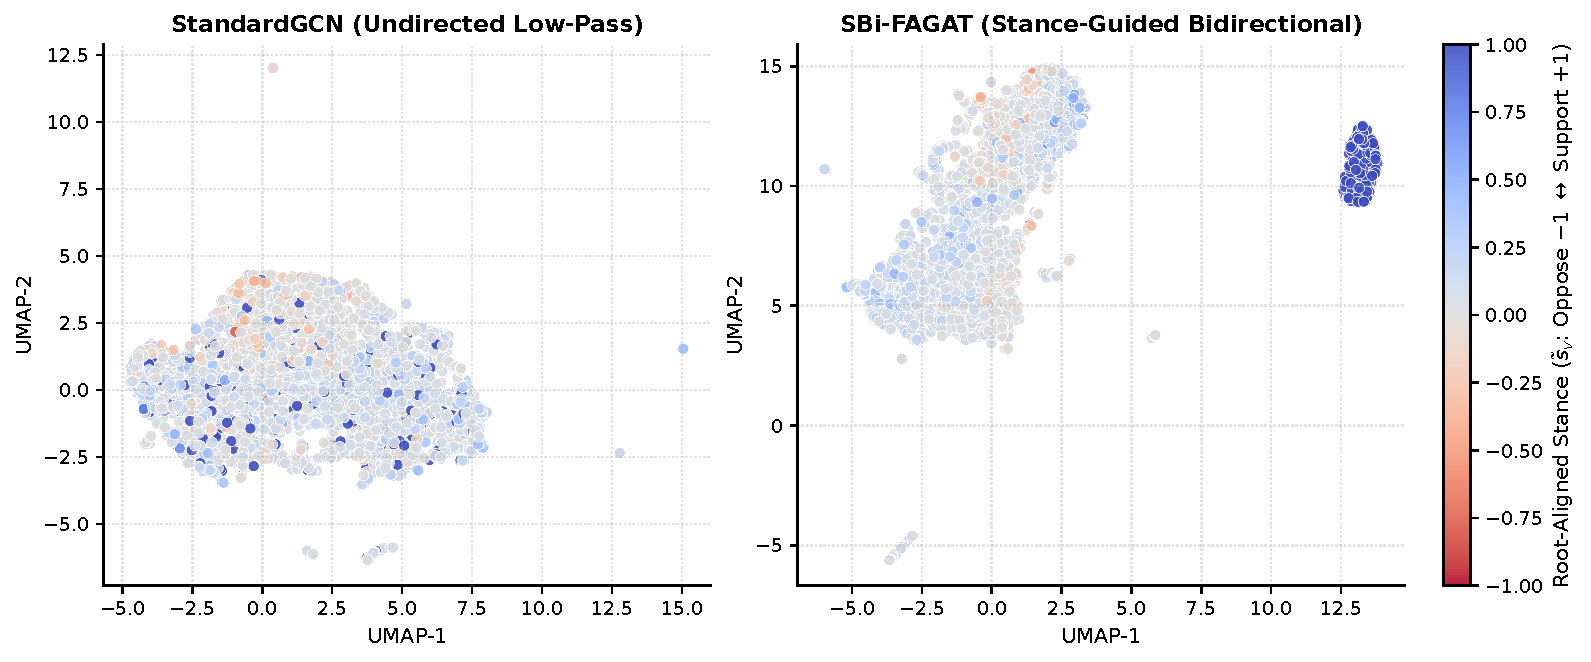
\includegraphics[width=\textwidth]{figures/pheme/fig1_umap_polarization.pdf}
\caption{PHEME Test-Split UMAP Node Embeddings: StandardGCN (left) vs.\ SBi-FAGAT (right), colored by causal root-aligned stance polarity on $\mathcal{V}_K$.}
\label{fig:umap_pheme}
\end{figure*}
}{}

\IfFileExists{figures/vn/fig1_umap_polarization.pdf}{
\begin{figure*}[t]
\centering
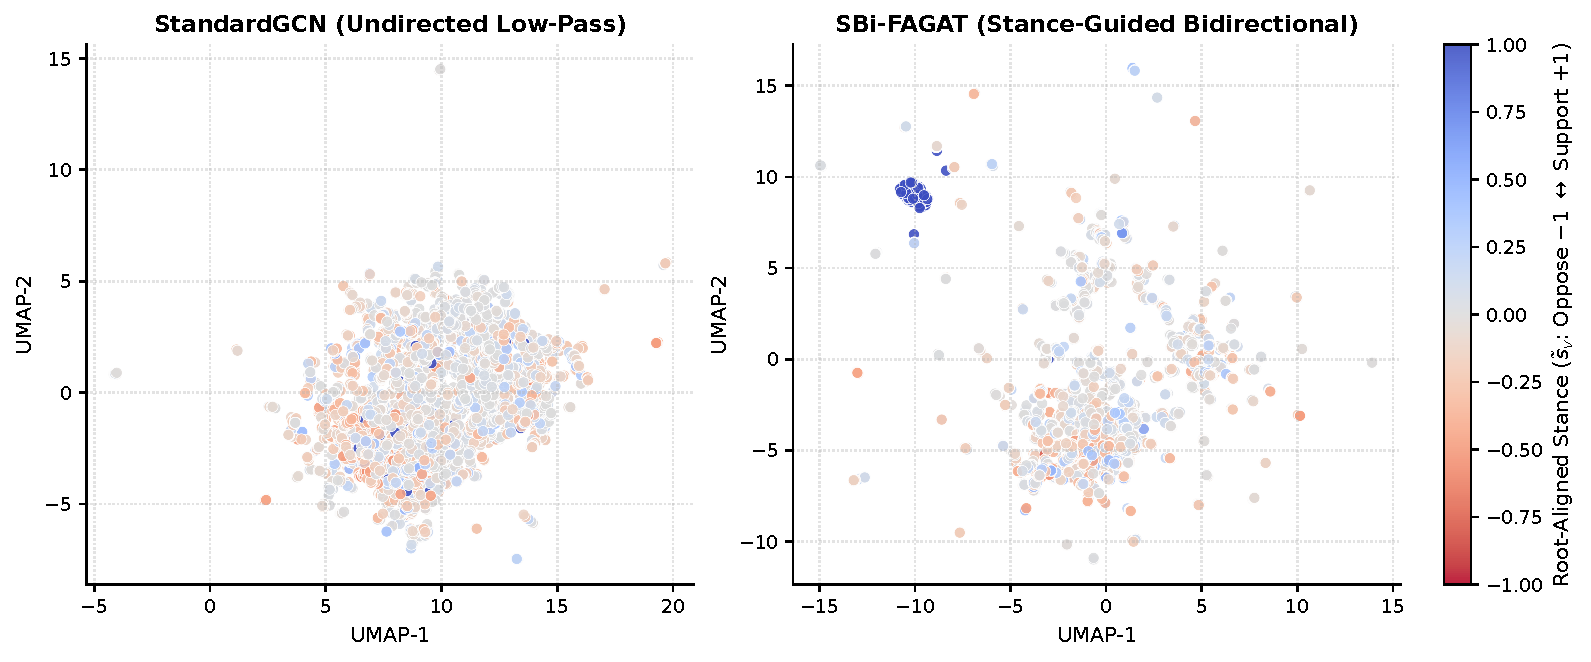
\includegraphics[width=\textwidth]{figures/vn/fig1_umap_polarization.pdf}
\caption{Vietnamese Reddit Test-Split UMAP Node Embeddings: StandardGCN (left) vs.\ SBi-FAGAT (right), colored by causal root-aligned stance polarity on $\mathcal{V}_K$.}
\label{fig:umap_vn}
\end{figure*}
}{}

\IfFileExists{figures/pheme/fig2_early_k_curve.pdf}{
\begin{figure*}[t]
\centering
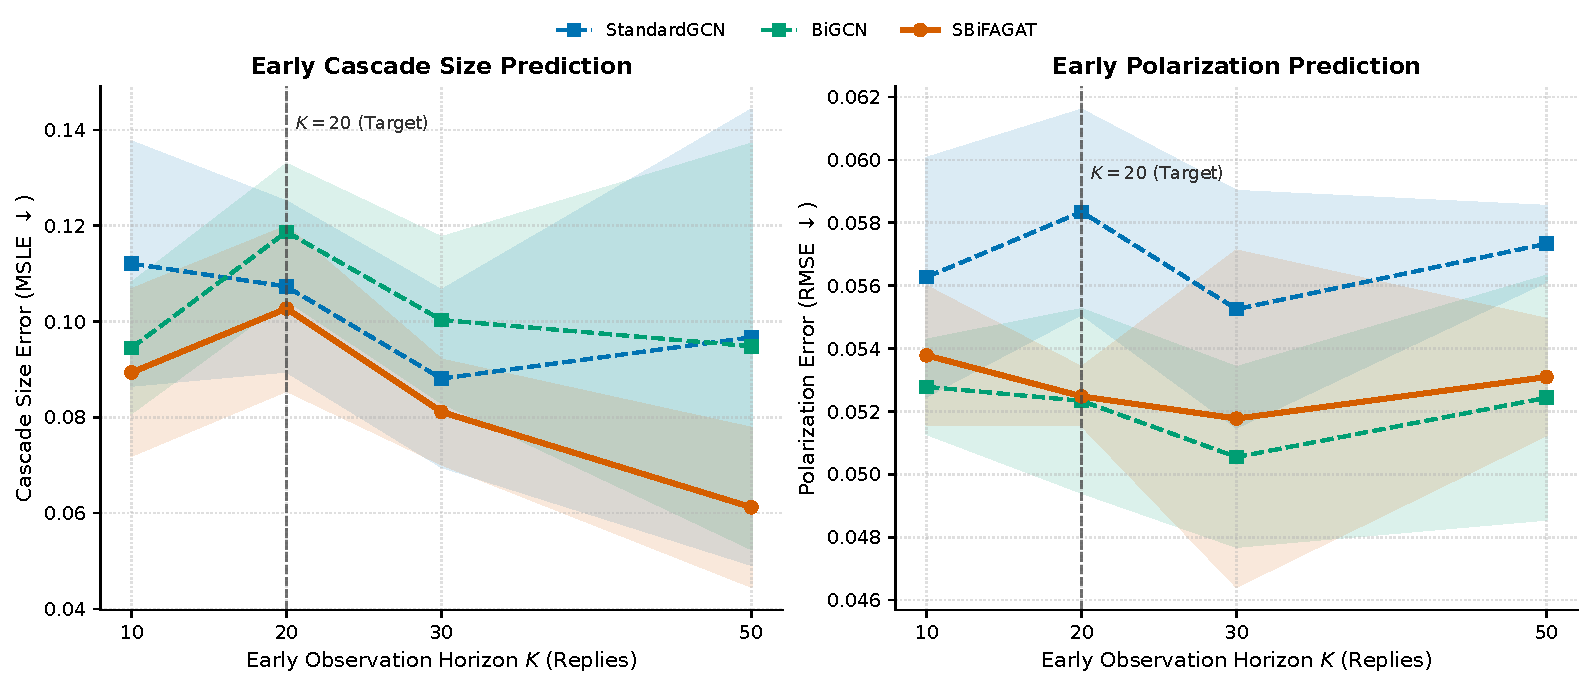
\includegraphics[width=\textwidth]{figures/pheme/fig2_early_k_curve.pdf}
\caption{PHEME Early Observation Horizon Sensitivity ($K \in \{10, 20, 30, 50\}$) evaluated on a common subset against a fixed future target window.}
\label{fig:k_curve_pheme}
\end{figure*}
}{}

\IfFileExists{figures/vn/fig2_early_k_curve.pdf}{
\begin{figure*}[t]
\centering
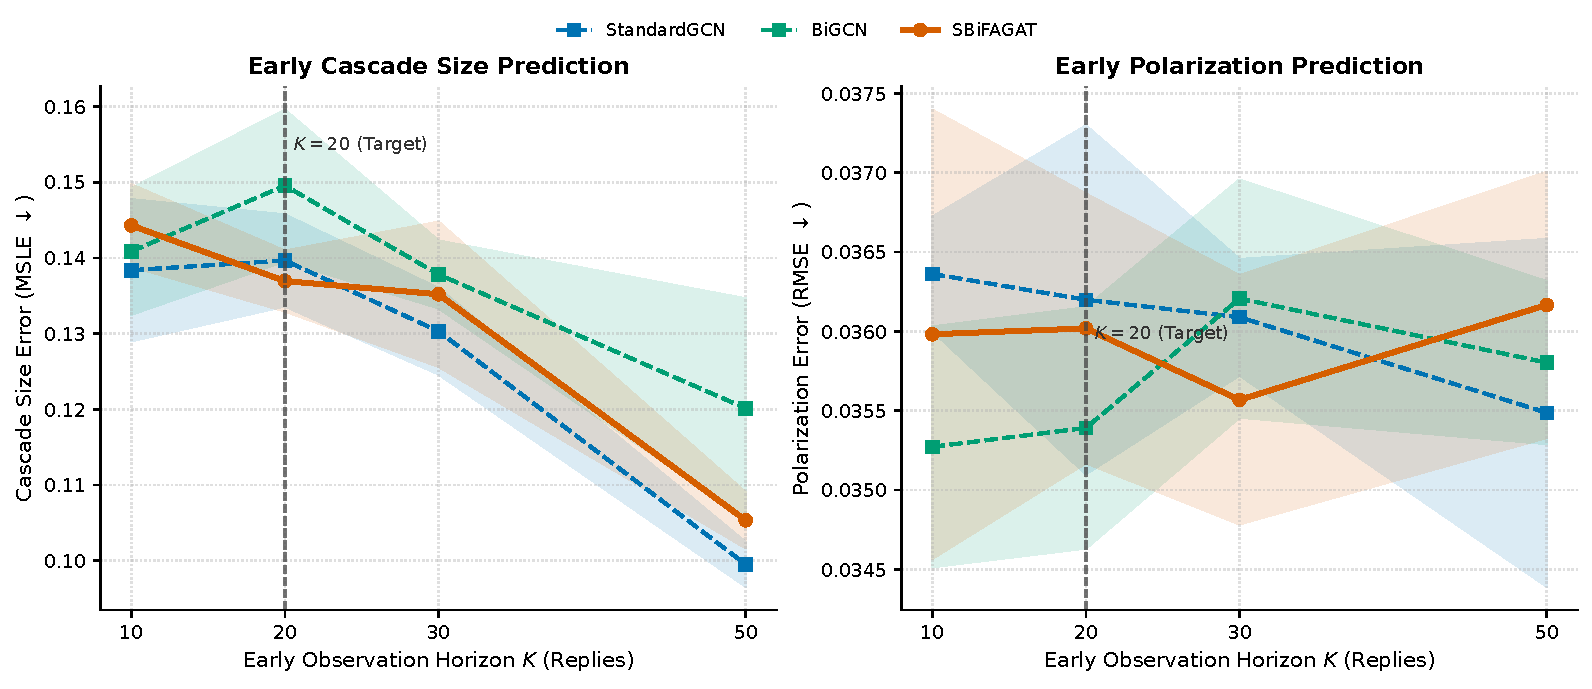
\includegraphics[width=\textwidth]{figures/vn/fig2_early_k_curve.pdf}
\caption{Vietnamese Reddit Early Observation Horizon Sensitivity ($K \in \{10, 20, 30, 50\}$) evaluated on a common subset against a fixed future target window.}
\label{fig:k_curve_vn}
\end{figure*}
}{}

\section{Case Study and Limitations}
\subsection{Trigger Comment Analysis}
For qualitative interpretability, \texttt{extract\_edge\_gates} ranks edges by gate magnitude $|\gamma_{uv}|$ and signed conflict polarity, exporting cascade tree heatmaps alongside top trigger comments (\texttt{fig3\_top5\_trigger\_comments.txt}).

\IfFileExists{figures/pheme/fig3_cascade_heatmap.pdf}{
\begin{figure*}[t]
\centering
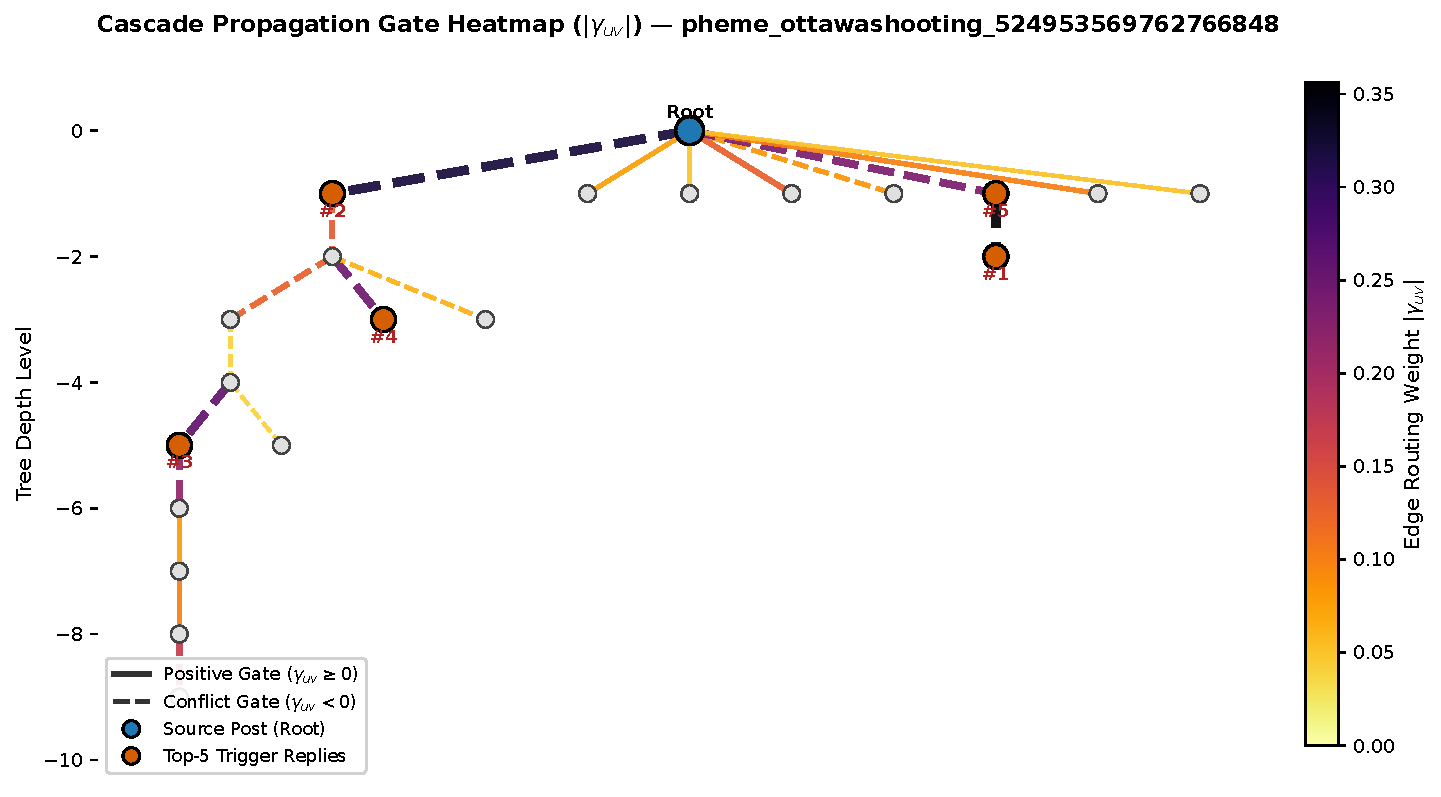
\includegraphics[width=0.92\textwidth]{figures/pheme/fig3_cascade_heatmap.pdf}
\caption{PHEME High-Polarization Cascade Gate Heatmap showing $|\gamma_{uv}|$ importance and signed polarity across early replies.}
\label{fig:heatmap_pheme}
\end{figure*}
}{}

\IfFileExists{figures/vn/fig3_cascade_heatmap.pdf}{
\begin{figure*}[t]
\centering
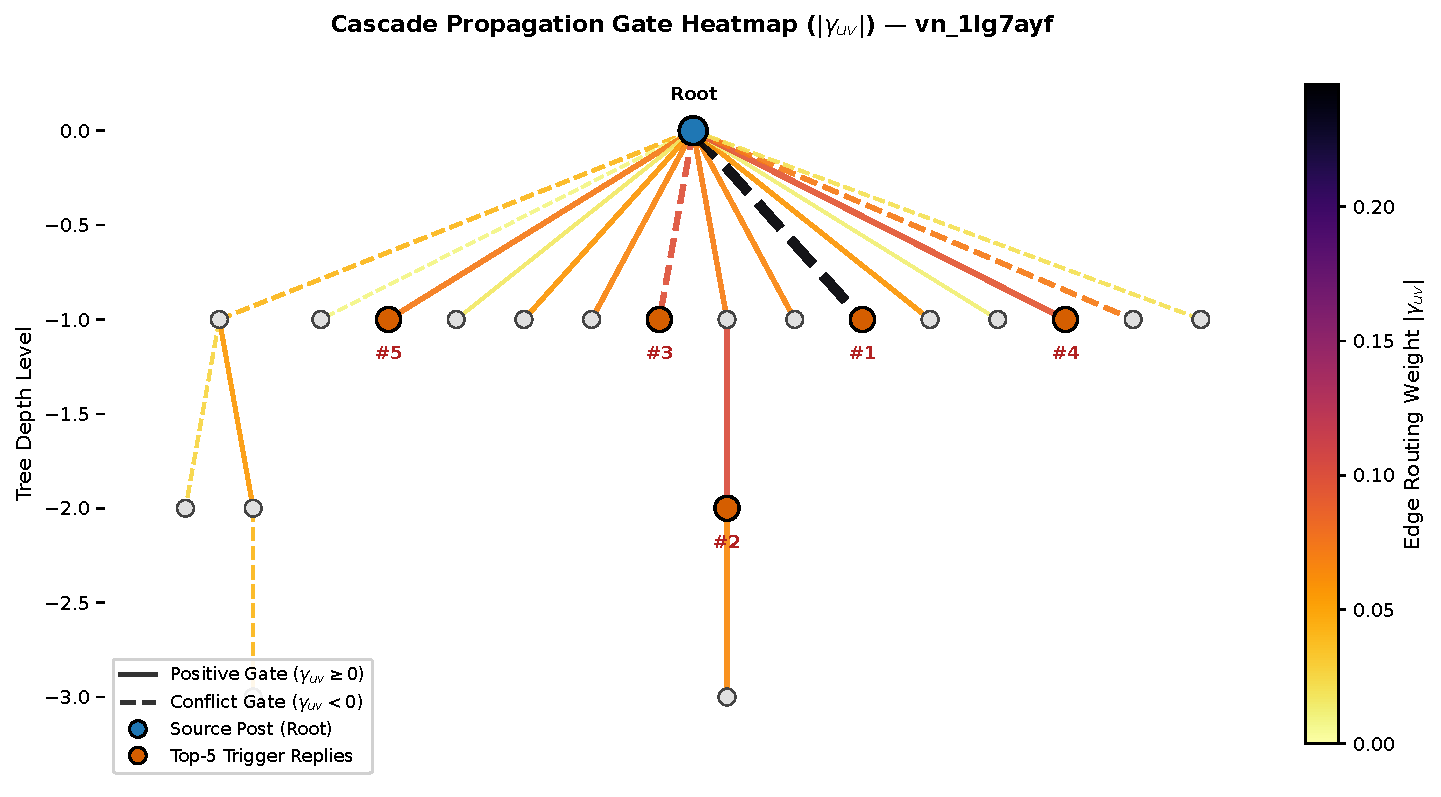
\includegraphics[width=0.92\textwidth]{figures/vn/fig3_cascade_heatmap.pdf}
\caption{Vietnamese Reddit High-Polarization Cascade Gate Heatmap showing $|\gamma_{uv}|$ importance and signed polarity across early replies.}
\label{fig:heatmap_vn}
\end{figure*}
}{}

\subsection{Observational Edge-Feature Sensitivity Analysis}
To examine how early affective incivility and ideological disagreement relate to model predictions beyond black-box accuracy, \texttt{scripts/analyze\_mechanisms.py} conducts empirical regime stratification (low conflict, civil disagreement, hostile conflict), trigger-edge depth profiling ($d=1$ vs.\ $d \ge 2$), and non-mutating input-feature sensitivity perturbations on trained test checkpoints. Generated LaTeX summaries and paired bootstrap shift plots are reported strictly as observational model-sensitivity associations rather than causal intervention effects.

\IfFileExists{tables_mechanisms_pheme.tex}{
  \begin{table*}[t]
\centering
\caption{Counterfactual Moderation Stress Test on PHEME Test Cascades (Mean Shift with 95\% Paired Bootstrap CI).}
\label{tab:mechanisms_pheme}
\begin{tabular}{lcccc}
\toprule
Counterfactual Intervention & All Test $\Delta \hat{y}_{\mathrm{size}}$ & All Test $\Delta \hat{y}_{\mathrm{polar}}$ & Q75+ $\Delta \hat{y}_{\mathrm{size}}$ & Q75+ $\Delta \hat{y}_{\mathrm{polar}}$ \\
\midrule
Cool Top-3 Trigger Hostility & $-0.0081$ $[-0.0110, -0.0053]$ & $-0.0001$ $[-0.0002, -0.0001]$ & $-0.0108$ $[-0.0177, -0.0048]$ & $-0.0003$ $[-0.0006, -0.0001]$ \\
Cool All Early Hostility & $-0.0193$ $[-0.0234, -0.0154]$ & $-0.0004$ $[-0.0005, -0.0003]$ & $-0.0222$ $[-0.0311, -0.0142]$ & $-0.0007$ $[-0.0011, -0.0003]$ \\
Neutralize Top-3 Trigger Conflict & $-0.0068$ $[-0.0097, -0.0037]$ & $-0.0001$ $[-0.0002, -0.0000]$ & $-0.0096$ $[-0.0165, -0.0033]$ & $-0.0003$ $[-0.0006, -0.0001]$ \\
Neutralize All Opposition & $-0.0099$ $[-0.0140, -0.0057]$ & $-0.0002$ $[-0.0004, -0.0001]$ & $-0.0155$ $[-0.0259, -0.0062]$ & $-0.0007$ $[-0.0011, -0.0002]$ \\
\bottomrule
\end{tabular}
\end{table*}

}{}

\IfFileExists{tables_mechanisms_vn.tex}{
  \begin{table*}[t]
\centering
\caption{Counterfactual Moderation Stress Test on VN Test Cascades (Mean Shift with 95\% Paired Bootstrap CI).}
\label{tab:mechanisms_vn}
\begin{tabular}{lcccc}
\toprule
Counterfactual Intervention & All Test $\Delta \hat{y}_{\mathrm{size}}$ & All Test $\Delta \hat{y}_{\mathrm{polar}}$ & Q75+ $\Delta \hat{y}_{\mathrm{size}}$ & Q75+ $\Delta \hat{y}_{\mathrm{polar}}$ \\
\midrule
Cool Top-3 Trigger Hostility & $+0.0024$ $[+0.0017, +0.0033]$ & $-0.0000$ $[-0.0001, -0.0000]$ & $+0.0025$ $[+0.0012, +0.0042]$ & $-0.0000$ $[-0.0001, -0.0000]$ \\
Cool All Early Hostility & $+0.0048$ $[+0.0037, +0.0058]$ & $-0.0001$ $[-0.0001, -0.0001]$ & $+0.0043$ $[+0.0024, +0.0065]$ & $-0.0001$ $[-0.0001, -0.0000]$ \\
Neutralize Top-3 Trigger Conflict & $+0.0036$ $[+0.0023, +0.0050]$ & $-0.0001$ $[-0.0001, -0.0001]$ & $+0.0028$ $[+0.0006, +0.0054]$ & $-0.0001$ $[-0.0001, -0.0000]$ \\
Neutralize All Opposition & $+0.0154$ $[+0.0127, +0.0181]$ & $-0.0004$ $[-0.0004, -0.0003]$ & $+0.0150$ $[+0.0080, +0.0215]$ & $-0.0003$ $[-0.0005, -0.0002]$ \\
\bottomrule
\end{tabular}
\end{table*}

}{}

\IfFileExists{figures/pheme/fig4_counterfactual_interventions.pdf}{
\begin{figure*}[t]
\centering
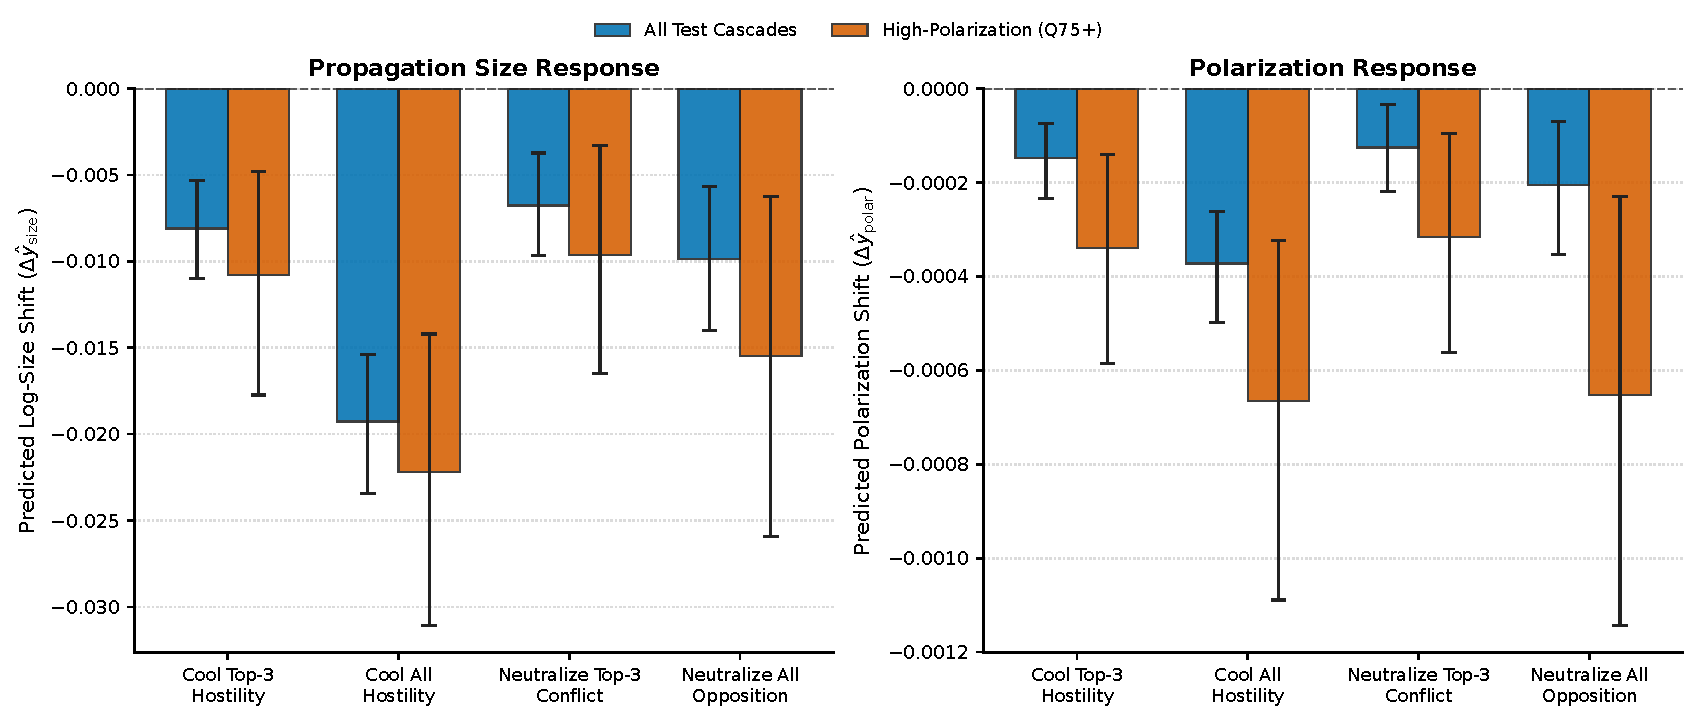
\includegraphics[width=0.92\textwidth]{figures/pheme/fig4_counterfactual_interventions.pdf}
\caption{PHEME Observational Edge-Feature Sensitivity Analysis: predicted cascade size ($\Delta\hat{y}_{\mathrm{size}}$) and polarization ($\Delta\hat{y}_{\mathrm{polar}}$) shifts under edge-attribute perturbation across All Test and High-Polarization (Q75+) cohorts with 95\% paired bootstrap confidence intervals (non-causal sensitivity probe).}
\label{fig:cf_pheme}
\end{figure*}
}{}

\IfFileExists{figures/vn/fig4_counterfactual_interventions.pdf}{
\begin{figure*}[t]
\centering
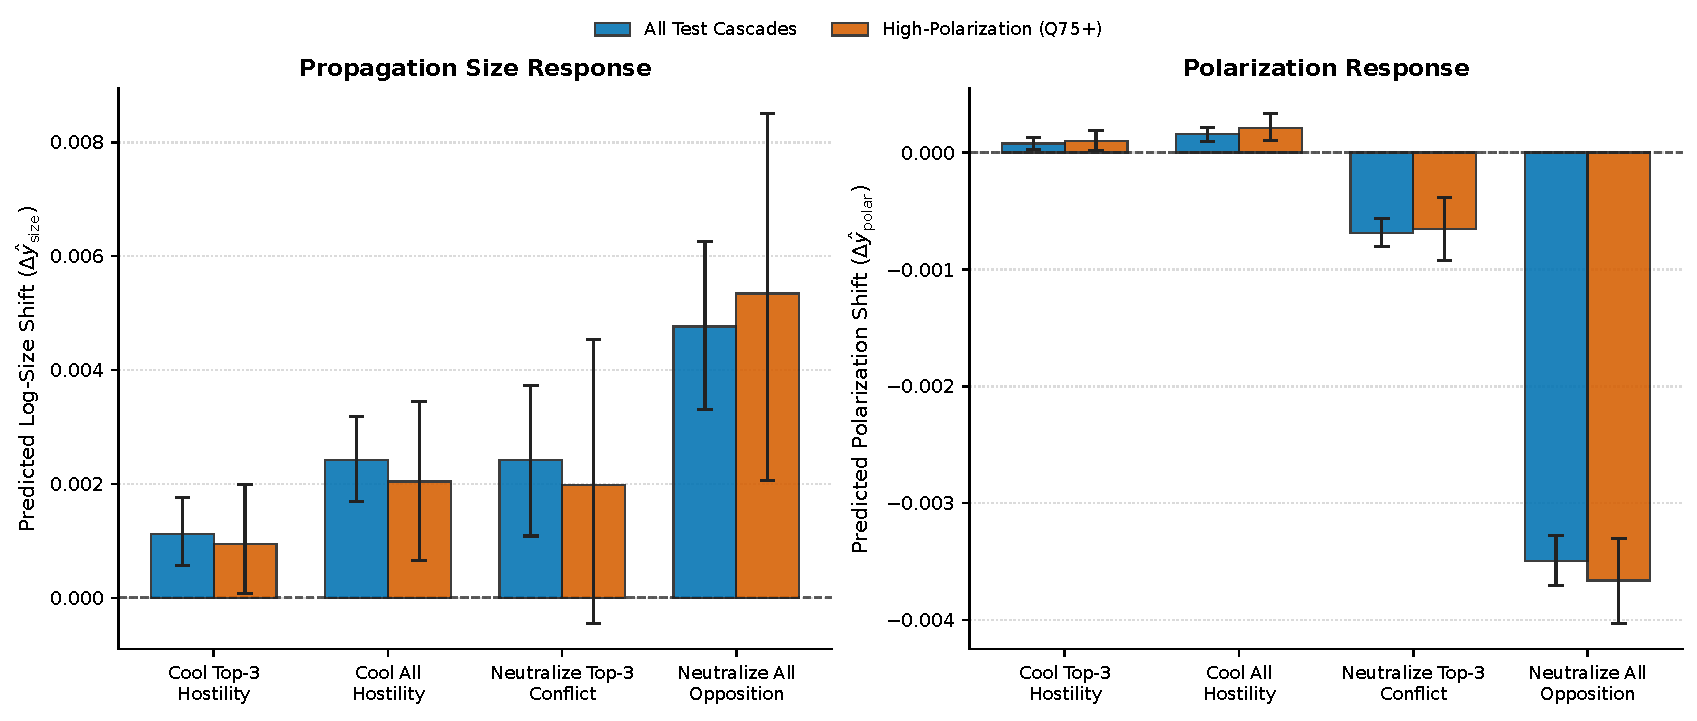
\includegraphics[width=0.92\textwidth]{figures/vn/fig4_counterfactual_interventions.pdf}
\caption{Vietnamese Reddit Observational Edge-Feature Sensitivity Analysis: predicted cascade size ($\Delta\hat{y}_{\mathrm{size}}$) and polarization ($\Delta\hat{y}_{\mathrm{polar}}$) shifts under edge-attribute perturbation across All Test and High-Polarization (Q75+) cohorts with 95\% paired bootstrap confidence intervals (non-causal sensitivity probe).}
\label{fig:cf_vn}
\end{figure*}
}{}

\subsection{Methodological Limitations and Ethical Safeguards}
We explicitly acknowledge four methodological constraints:
\begin{itemize}
    \item \textbf{Early Cascade Scale vs.\ Macro Echo Chambers:} Each observed graph models an isolated discussion cascade up to $|\mathcal{V}_K| \le 21$ nodes using intra-cascade structural-temporal descriptors rather than a cross-topic longitudinal user-interaction graph; consequently, SBi-FAGAT captures thread-level ideological and affective polarization rather than macro-level community echo chambers, which remain left for future work. Likewise, external UPFD transfer experiments reflect post-hoc text-free structural propagation (without linguistic early-reply features) rather than early discourse polarization.
    \item \textbf{Silver-Standard Polarization Label \& Gate 1 Audit Scope:} $y_{\text{polar}}$ (linear-amplitude scale) is derived from NLP stance models over future interactions rather than exhaustive manual tree annotation. English stance reliability uses the external RumourEval SDQC benchmark, while Vietnamese reliability is structured around a streamlined 20-pair pilot calibration, 120-pair Test dual-annotator audit (3-class stance and binary \texttt{clean} vs.\ \texttt{uncivil} reply incivility with inverse-propensity weighting and ROC-AUC/PR-AUC via \texttt{scripts/compute\_kappa.py}), and 30 held-out Test trees (0--4 Likert grading evaluated with Kendall $\tau_b$ and AUROC $@ \ge 2$ via \texttt{scripts/audit\_vn\_50\_trees.py}), alongside construct validity against Sarle's Bimodality Coefficient, signed assortativity, and Early-$K$ Persistence comparison; human scoring of these exported blind VN sheets remains active in Gate 1.
    \item \textbf{Heuristic VN Split \& Pending Track 2 v3 Re-Execution:} Lacking exogenous news event IDs on Reddit Vietnam, canonical Train/Val/Test separation uses 30-day temporal windows and TF-IDF cosine ($\ge 0.30$) clustering, cross-checked via a chronological temporal holdout (\texttt{edge\_source="teacher"}, Table~\ref{tab:temporal_vn}). Current \texttt{tables\_*\_pheme.tex} reflect the prior quadratic-target $K=20, N_{\text{reply}} \ge 25$ Kaggle Cohort B archive (\texttt{min\_total\_replies\_extracted=25}) pending optional \texttt{min\_total\_replies=15} feature re-extraction for Track 2 v3 ($K=10, N_{\text{reply}} \ge 15$) GPU execution.
    \item \textbf{Privacy Preservation \& Data Hygiene:} User identifiers are pseudonymized via salted SHA-256 hashing prior to persistence, personal PII (phone numbers, national IDs, bank accounts, personal Facebook profiles), doxxing posts, and crypto spam are automatically redacted or filtered prior to storage and blind audit export, and sealed answer-key audit files are excluded from distribution archives.
\end{itemize}

\section{Conclusion}
We presented SBi-FAGAT under a unified, leakage-checked 2D bilingual architecture combining Ancestor-Conditioned SpanPool node representations, reply-span-pooled stance--hostility distillation, dual-channel Top-Down/Bottom-Up signed graph attention, and KL-calibrated multi-task optimization. Following GPU execution on full PHEME and Vietnamese Reddit splits and human reliability audits, generated LaTeX tables and vector figures integrate directly into this IEEEtran manuscript via \texttt{scripts/assemble\_paper\_artifacts.py}.

\bibliographystyle{IEEEtran}
\bibliography{references}

\end{document}
